%---------------------%
\subsection{High-level components and their interaction}
In the following section it is provided a high level view of the architecture of the system, which is structured following the three logic layer:\\

\begin{figure}[H]
    \begin{center}
    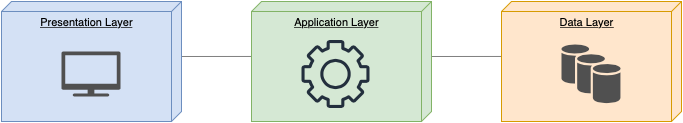
\includegraphics[width=1.2\textwidth]{images/System architecture.png}
    \caption{three layer architecture}
    \label{fig:system architecture}
    \end{center}
\end{figure}

\begin{itemize}
    \item \textbf{Presentation Layer (P)}: The presentation tier is the user interface and communication layer 
    of the application, where the end user interacts with the application. Its main purpose is to display 
    information to and collect information from the user. This top-level tier can run on a web browser, 
    as desktop application, or a graphical user interface (GUI), for example. \\ \\Web presentation tiers 
    are usually developed using HTML, CSS and JavaScript. Desktop applications can be written in a variety 
    of languages depending on the platform.
    \item \textbf{Business Logic or Application Layer(L)}: The application tier is the heart of the application. In this tier, information collected in the presentation tier is processed - sometimes against other information in the data tier - using business logic, a specific set of business rules. The application tier can also add, delete or modify data in the data tier.\\ \\The application tier is typically developed using Python, Java, Perl, PHP or Ruby, and communicates with the data tier using API calls. 
    \item \textbf{Data Layer (D)}: The data tier, sometimes called database tier, data access tier or back-end, is where the information processed by the application is stored and managed. This can be a relational database management system such as PostgreSQL, MySQL, MariaDB, Oracle, DB2, Informix or Microsoft SQL Server, or in a NoSQL Database server such as Cassandra, CouchDB or MongoDB. 
\end{itemize}

In this case the system is a distributed application that follows the client-server paradigm: it is a two-tier architecture, consisting of a presentation and a data tier. the business logic lives in the data tier only.
In a two-tier application, all communication goes through the application tier. The presentation tier and the data tier cannot communicate directly with one another. 

Client and server are being allocated into different physical machines and their communication takes place via other components and interfaces, located in the middle of the structure and composed by hardware and software modules. 
The client is a Web Application, with is by definition a thin client, because of its total dependency from the server; so it only contains the presentation layer.

\begin{figure}[H]
    \begin{center}
    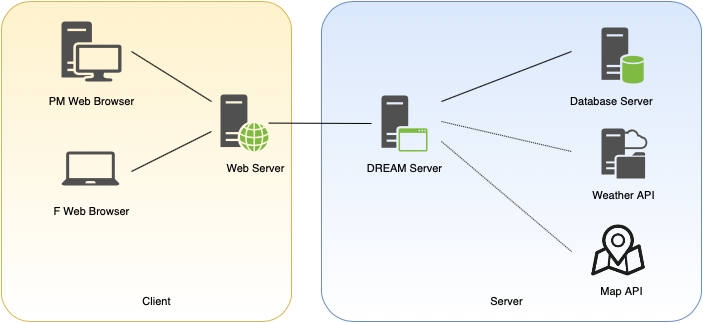
\includegraphics[width=1.2\textwidth]{images/System diagram.png}
    \caption{Dream system diagram.}
    \label{fig:system diagram}
    \end{center}
\end{figure}

\begin{itemize}
    \item \textbf{Server side:}
        \begin{itemize}
            \item \underline{ApplicationServer (DREAM Server)}: it is the central point of the system. Is a server whit all the application logic, that communicates with the other servers. 
            \item \underline{Database Server}: this is the server where all the application data are stored.
            \item \underline{Weather API}: external API used to retrieve data about weather in the territory. This information will be used to fill each farm page.
            \item \underline{Map API}: external API used to retrieve data about the territory.
        \end{itemize}
    \item \textbf{Client side:}
        \begin{itemize}
            \item \underline{Policy Maker Web Browser}: browser used by the policy maker from their work desk to access to the system
            \item \underline{Farmer Web Browser}: browser used by the farmer to access to the system
        \end{itemize}
\end{itemize}


%---------------------%
\subsection{Component view}

In this section it is provided a description of the components and interfaces of the system, how they are organized internally and how they communicate with each other.

\subsubsection{High Level}

\begin{figure}[H]
    \begin{center}
    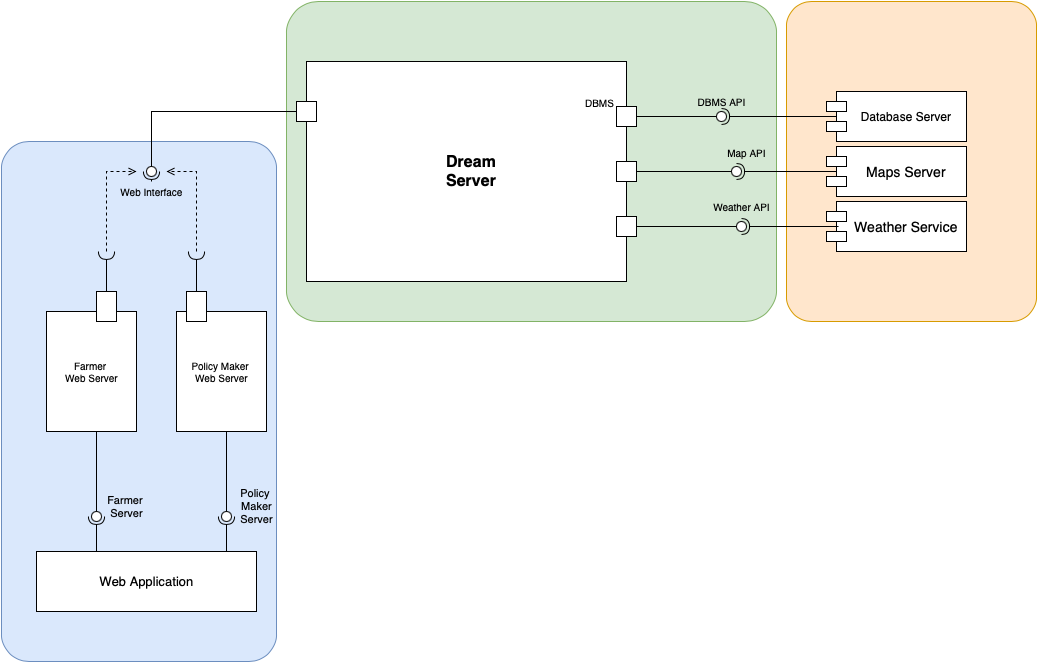
\includegraphics[width=1\textwidth]{images/Component3.png}
    \caption{Component view.}
    \label{fig:component view2}
    \end{center}
\end{figure}

\begin{itemize}
    \item \textbf{Dream Server}: this component contains the hole application logic of the system. The interfaces it provides allow the user, both farmer and policy maker, to comunicate with the server; them also allow the server to interact with external system that provide different kind of data.
    \item \textbf{Web Application}: it rapresents the web application reachable by any web browser. It is the first component that any user uses to connect with the system.
    \item \textbf{Farmer Web Server}: it provides the interface to a farmer to interact with the system. It has the minimum logic to make visible the content of the application provided by the server of the system. 
    \item \textbf{PolicyMaker Web Server}: the same as the one above but specific for the policy maker.
    \item \textbf{Database Server}: it provides the interfaces in all the processes that need to require or store information from the database of the system
    \item \textbf{Maps Server}: it provides the interfaces when the Dream server needs the maps data to make it visible and fill it with all the farms in the sistem, locating them by the position provided from their owner in the registration phase.
    \item \textbf{Weather Server}: it provides the interfaces to Dream server to retreive weather data of the territory.
\end{itemize}

\subsubsection{Server}
More specific and detailed on the server inner components.

\begin{figure}[H]
    \begin{center}
    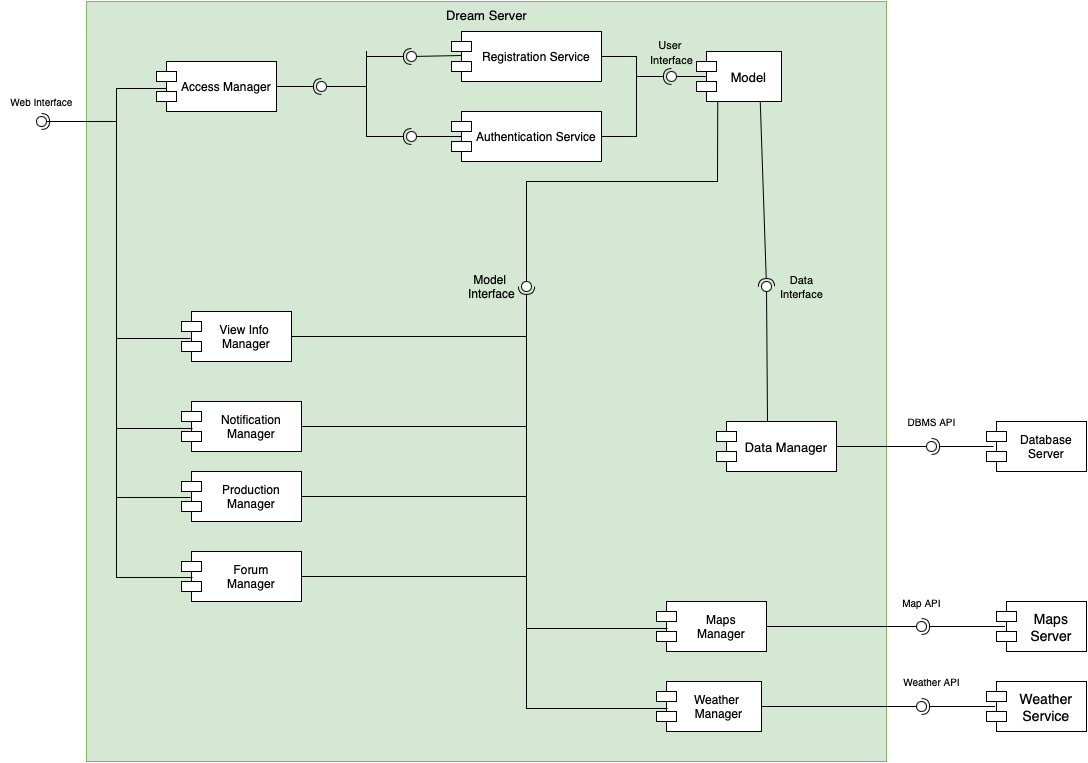
\includegraphics[width=1\textwidth]{images/ServerComponent3.png}
    \caption{Inner server component view2.}
    \label{fig:server component view2}
    \end{center}
\end{figure}

\begin{itemize}
    \item \textbf{Access Manager}: this component provide the Web interface to the user and make login and sign up opratation possible. It recognize the operation required and if it is permitted (sign up only for new farmers) comunicate with the right component that follow.
    \item \textbf{Registration Service}: if a request of a new registration occupr, it check the credential submitted by the new user and create the object that represent it, that will be stored in the Model; in fact it has an iterface to comunicate with the Model.
    \item \textbf{Authentication Service}: this component is called by the Access manager when an authentication request occur. In this case it collect the data about this specific user and verify if the credential submitted correspond. When them maches it let the user to access the system, otherwise generate an error signal.
    \item \textbf{ViewInfoManager}: this component is used by the system to collect the data from the Model request by the user. It operates when a farm's page has to be constructed with all the information visible in it.
    \item \textbf{Notification Manager}: this component has the ability to differ based on the notification it receives:
        \begin{itemize}
            \item advice: when a farmer submit this type of notification his only duty is the one to make possible the saving of it.
            \item help: when a farmer submit a request of help this component select randomly one policy maker (from the ones saved in the system) and send him the notification.
            \item solution: when a policy maker decides to respond to a request of help, he send this type of notification. This componenet forward it to the addressee.
            \item evaluation: when a policy maker evaluate a farm, this component takes care of sending it to the owner of the farm.
        \end{itemize}
    For all thee four type of notifications it attach the current day and time of the subbmission.
    This component also make possible to the user to visualize the list of all notifications received and, if asked, visualize in details the one selected.

    \item \textbf{Production Manager}: this component, by its connection to the model via \underline{Model interface}, povides all production data required for a specific farm. 
    \item \textbf{Forum Manager}: this component manage all the messages comunication between farmers via forum. It gets all the messages in it, saved as  List in the Model and comunicate to it the new ones, that has to mìbe saved (attaching to it the date and time).
    \item \textbf{Model}: this component have a main role in the system because it rapresents the data so all other components needs to interact with it, to ptovide the page and informations required.
    \item \textbf{Data Manager}: it manages all the process where data are needed by the system. It uses methods provided by the DBMS API to execute queries on the database and object-relational mapping to the Model.
    \item \textbf{Maps Manager}: this component is used to retreive map data, in order to provide a visualization of where each farmer registered in the system are located in the territory.
    \item \textbf{Weather Manager}: this component is used to retreive weather data specific in the position of the farms. It map to the Model the information from a relational to an object construct as a structure where the key is the farm position and in the value another structure to linked each day the weather and temperature.
\end{itemize}

%---------------------%
\subsection{Deployment view}
The deplyment diagram in figure .. shows the allocation of the software components in the physical tiers of the system. 
The system is organized into a three-tier application. This type of architecture can be 
beneficial because each tier can be developed in parallel and maintained as single modules on separate platforms.


\begin{itemize}
    \item \textbf{Presentation Tier}: it is the user interface of the application, where the user interacts with the application. 
    In this case it can only be a computer with a web browser running on an operating system (for example MacOS).
    It is composed by the web app an the web server. The web server is responsible for the communication between application server 
    and the client.

    \item \textbf{Application Tier}: it is the logic tier of the application. Where all the information 
    collected in the previous tier are processed using business logic. This tier is also 
    responsible for the communication with the data tier through the DBMS gateway.
    The most important thing is that all communication of the system goes through this tier.

    \item \textbf{Data Tier}: it is a database server for managing read and write access to the database. 
    Therefore all the information processed by the application tier are stored and managed here.
    Data tier is also independent of the two previous tiers. 
\end{itemize}
%---------------------%
\subsection{Runtime view}

In this section the focus is on the specific (dynamic) interaction between the components of the system; in other world the behaviour of the system at runtime.
The functionality offered by the component are the same as the ones in the RASD, but this time the focus is on how the internal components provides it.
(MAKE SURE THAT THE OPERATION AND COMPONENT ARE ALL DEFINED IN THE COMPONENT DIAG/VIEW, in particular the interfaces that receives the msg)

\begin{enumerate}
    \item \textbf{farmer registration}\\
    In this sequence diagram is shown the sign up operation by a new farmer. After the user fill the form provided by the web application with: name, surmane, farm's name, position, email and password. The Dream server stores all this information as a Farmer object in the Model, and also saves them in the database. At the end of the process redirects the user to the login page, only if some error occurred the data are not saved and the user is asked to repeat the operation.
    \begin{figure}[H]
        \begin{center}
        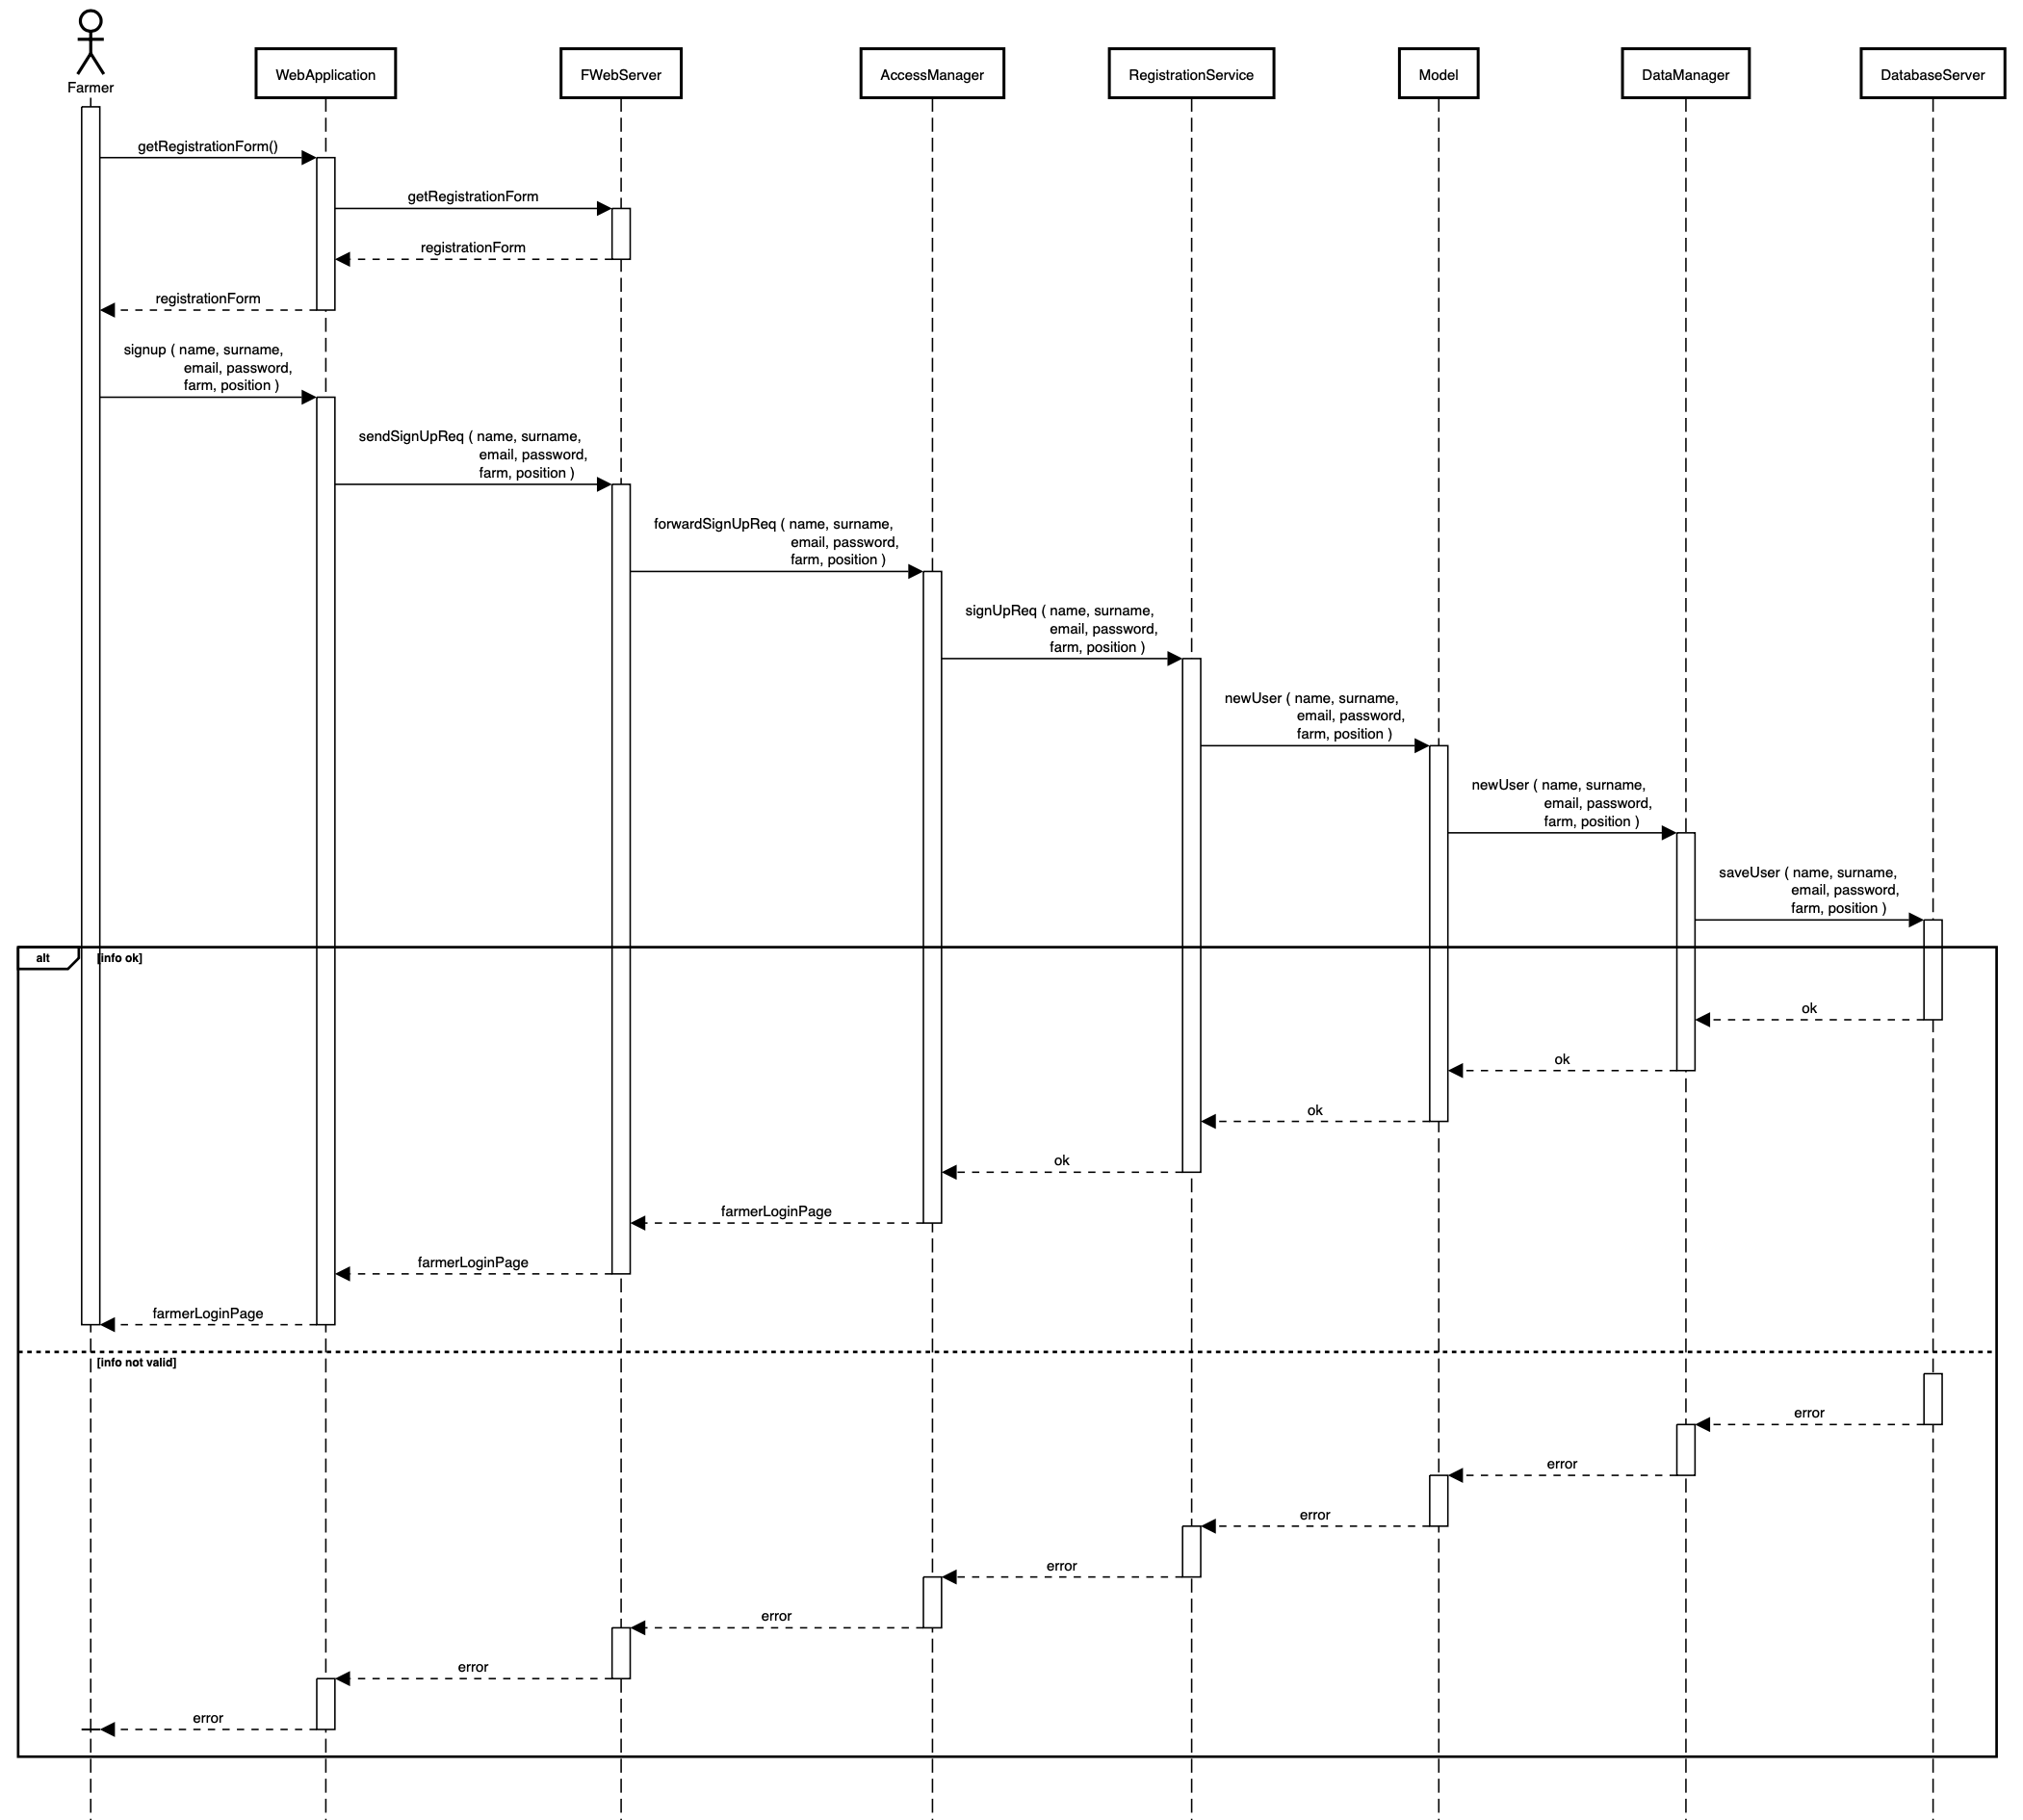
\includegraphics[width=0.7\textwidth]{sequance/signup.png}
        \caption{\emph{SignUp} sequence diagram}
        \label{fig:sequence1}
        \end{center}
    \end{figure}
    \item \textbf{login}\\
    In this sequence diagram the process of user login is shown, at first for the farmer and then for the policy maker. For both are almost the same, except that the farmers needs to provide email and password as access credentials and the policy maker a code and password. Another difference is in the server that forward the request to login to the Dream server component. If the credentials are wrong or missing the system gave an error message, if not the home page of the user is returned.
    \begin{figure}[H]
        \begin{center}
        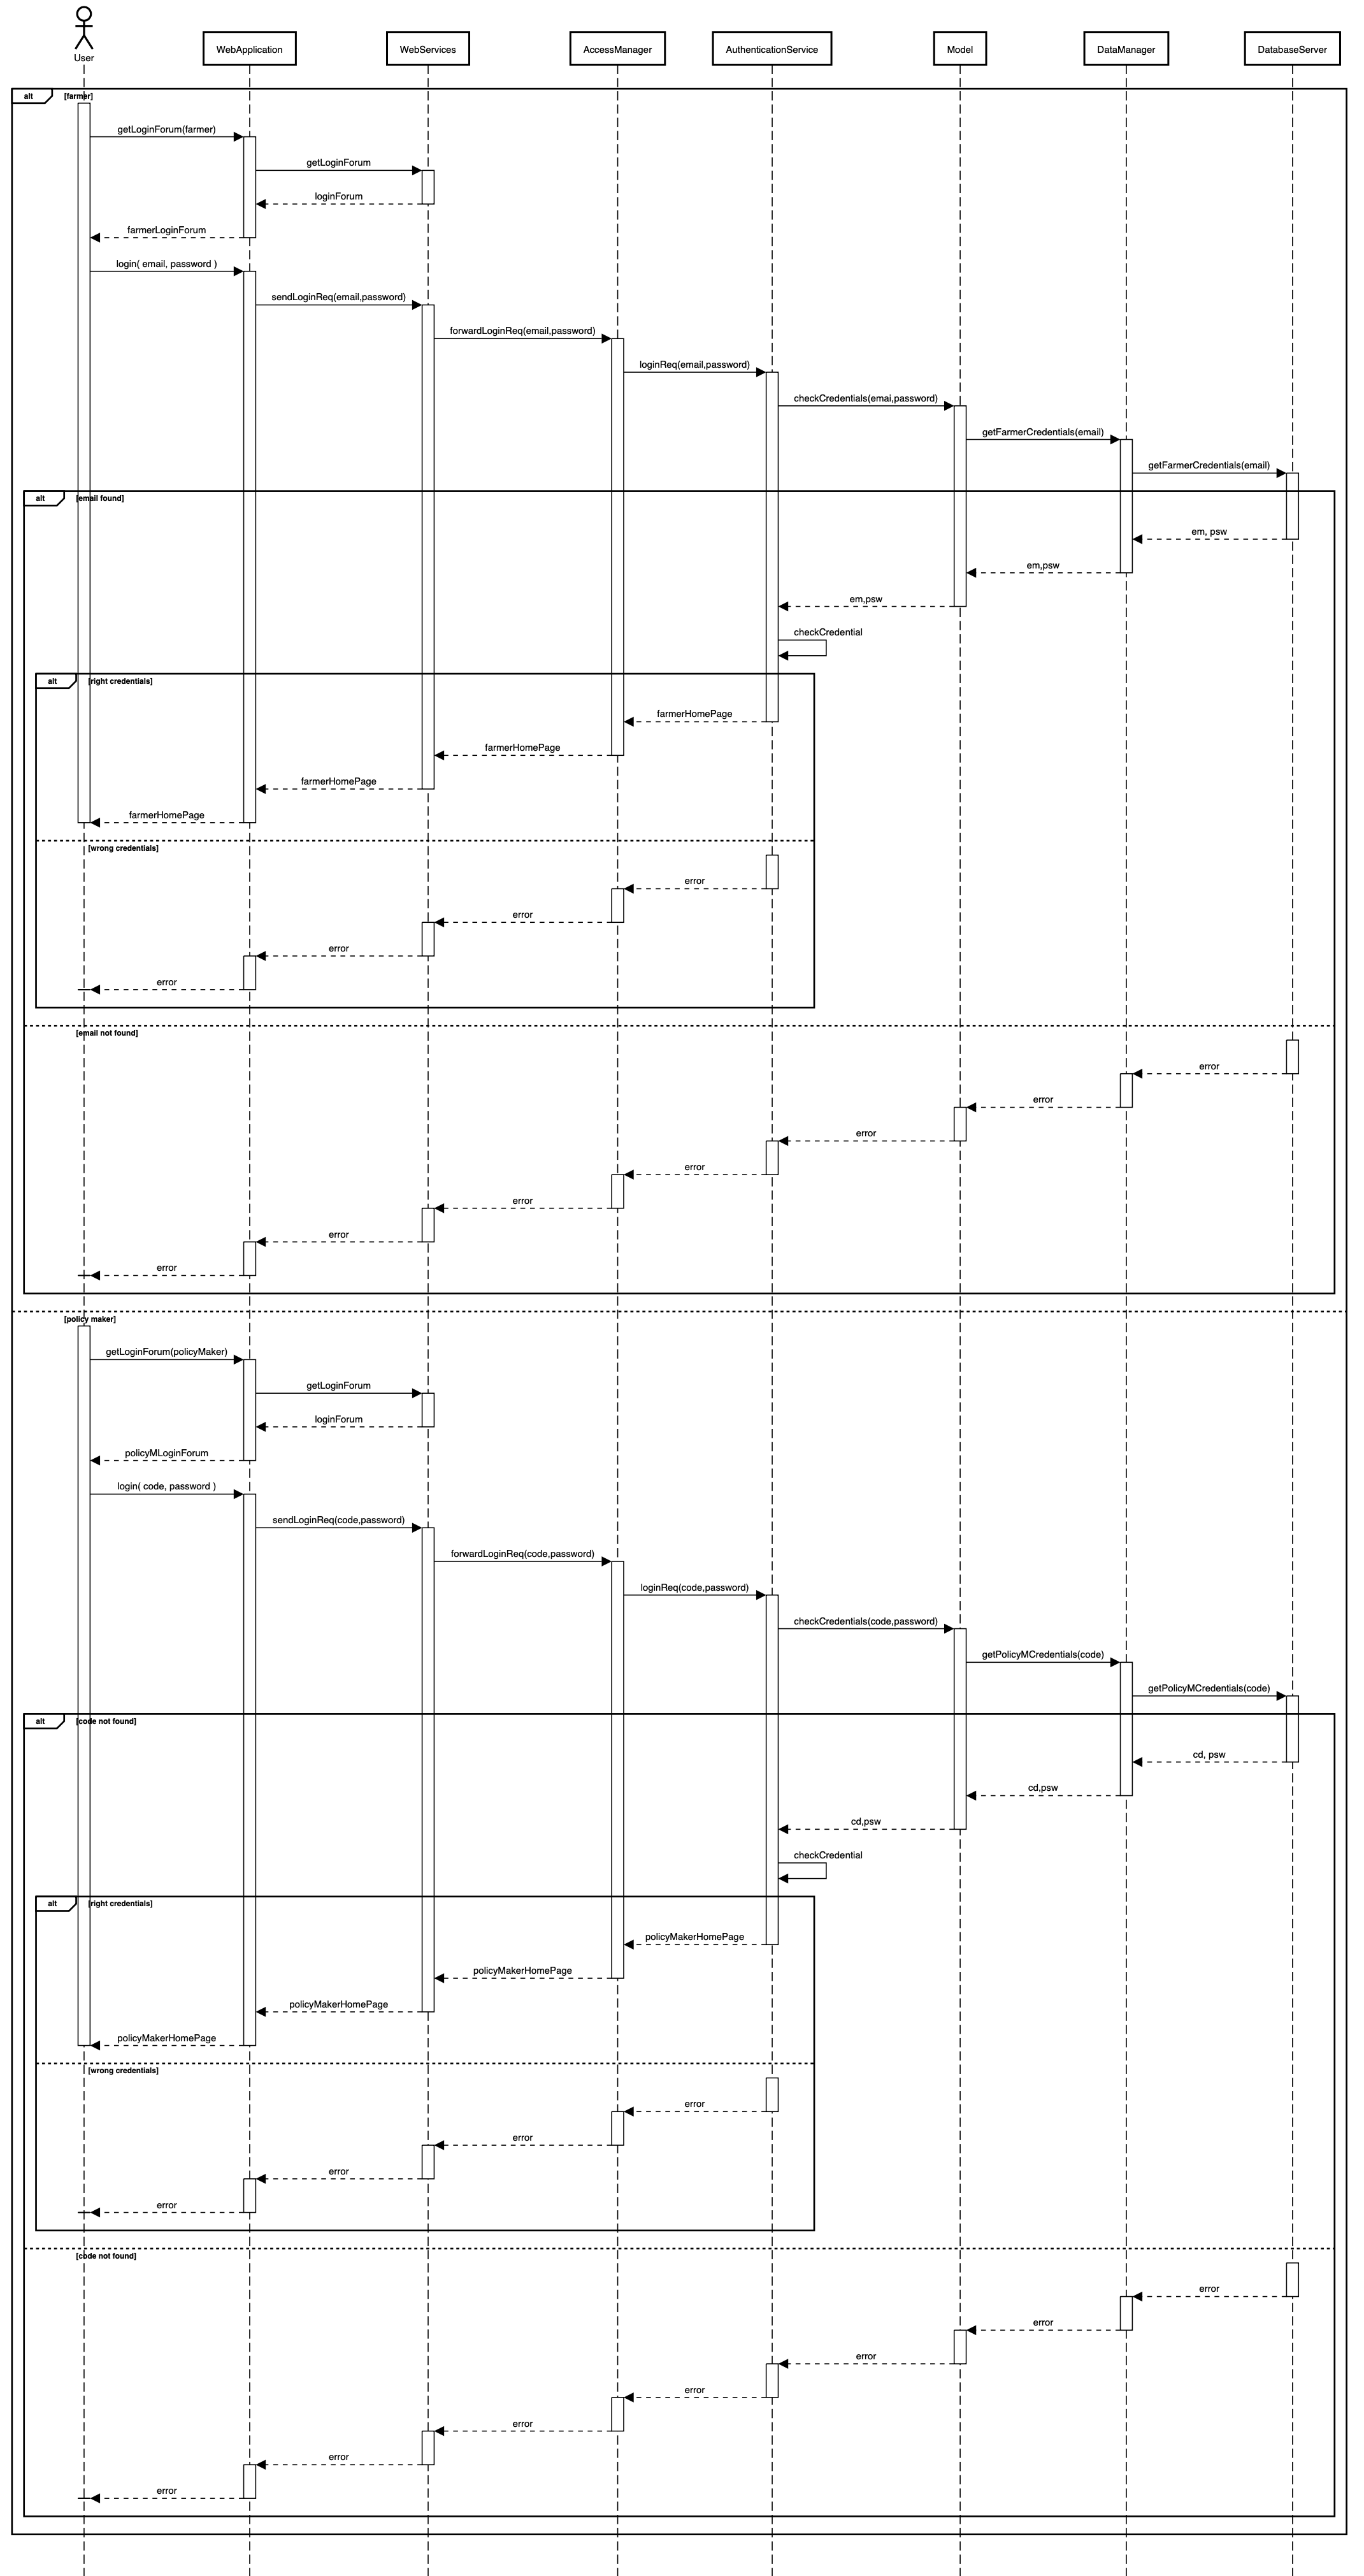
\includegraphics[width=0.7\textwidth]{sequance/login.png}
        \caption{\emph{Login} sequence diagram}
        \label{fig:sequence2}
        \end{center}
    \end{figure}
    \item \textbf{farmer read and write on forum}\\
    In this sequence is shown how the system provides the forum with all the messages yet sended after the request of a farmer and a form where he can write a message and a button to send it. As shown, due to the Forum Manager, when a message is send it is saved whit the references of the sender and the date and time. These addictonal information are used to sort the messages by the timestamp and specify the sender name near the message itself.
    \begin{figure}[H]
        \begin{center}
        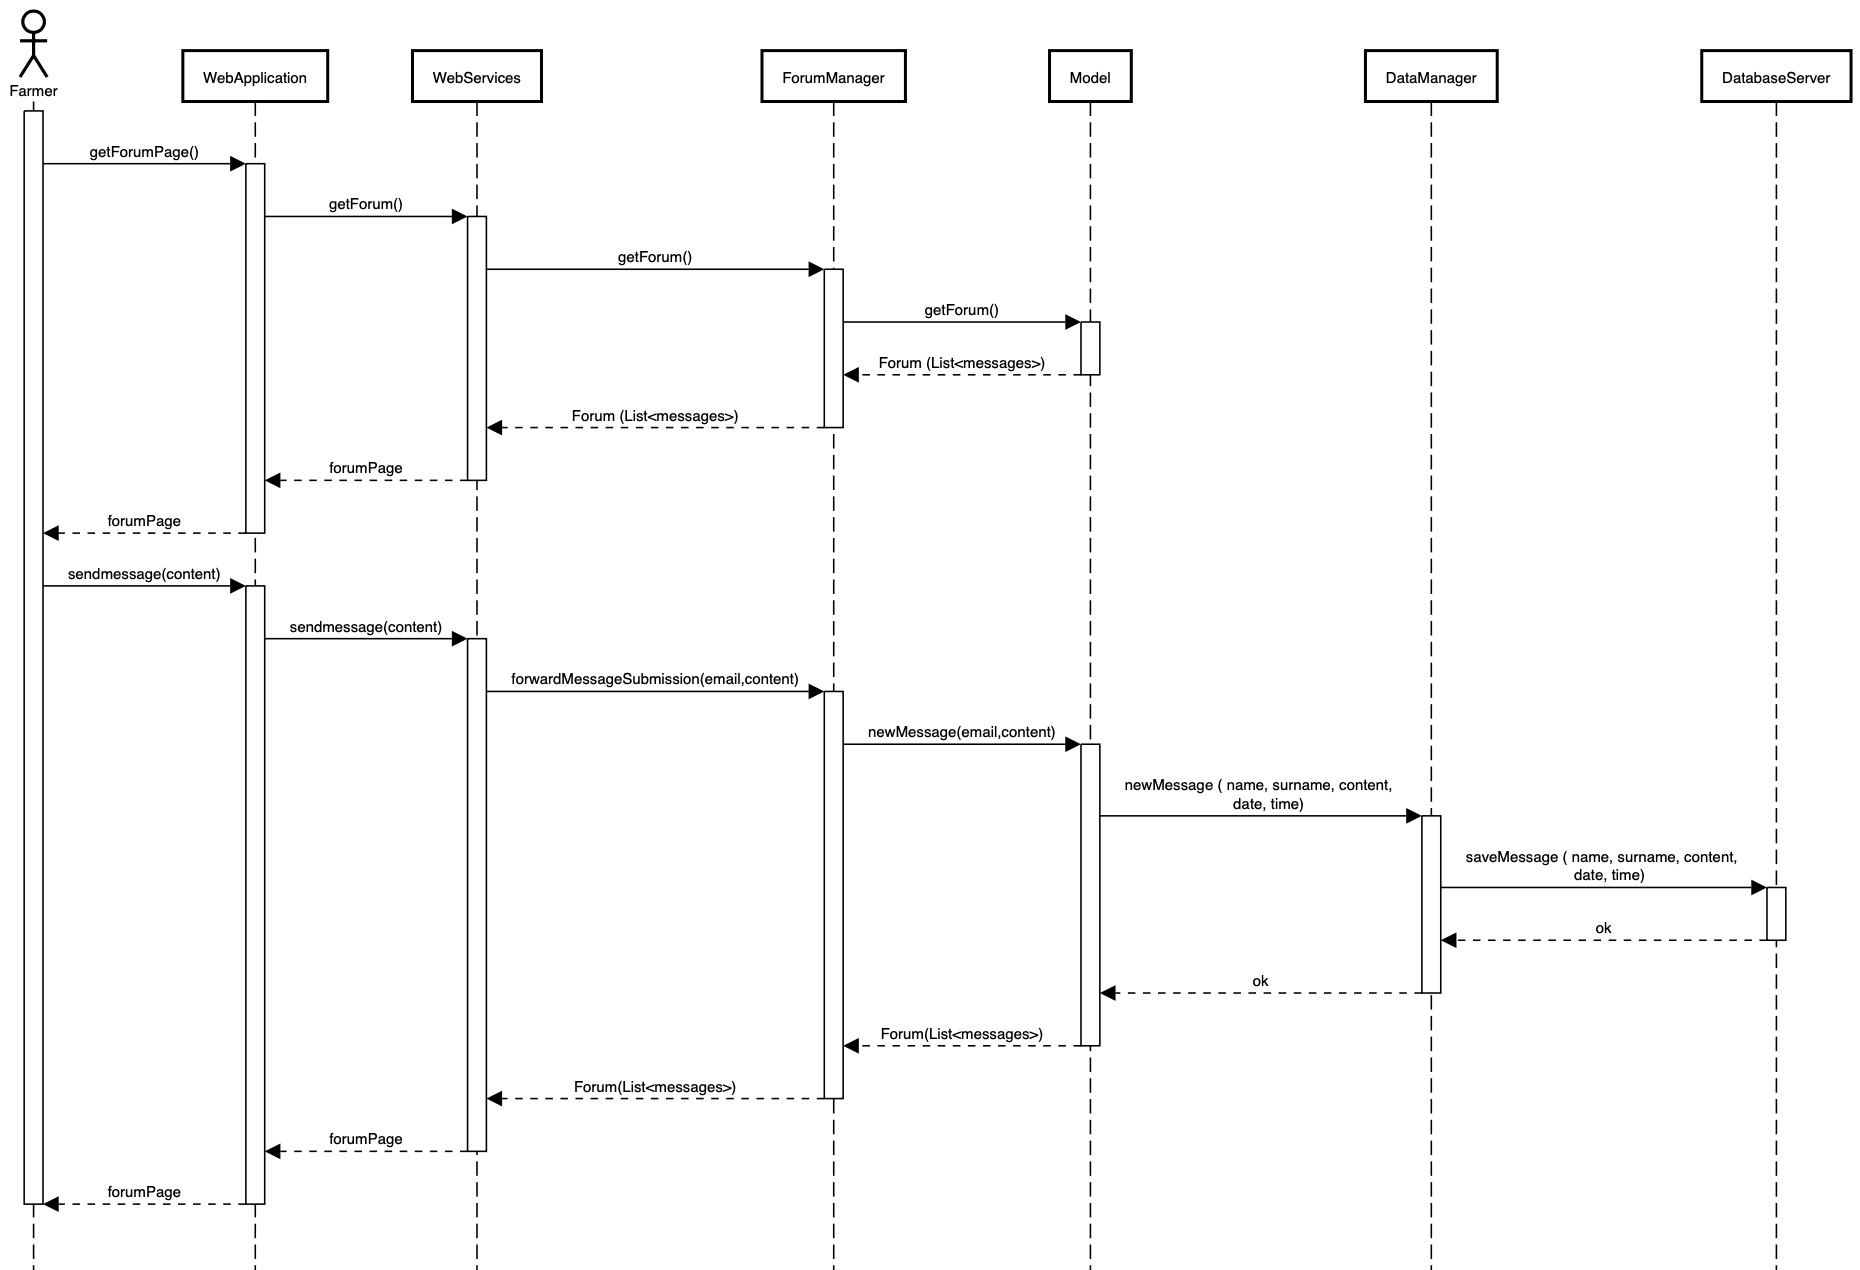
\includegraphics[width=0.7\textwidth]{sequance/forum.png}
        \caption{\emph{Save message} sequence diagram}
        \label{fig:sequence3}
        \end{center}
    \end{figure}
    \item \textbf{farmer submit production data}\\
    Here is shown how a farmer can submit new information about his production. The Web Application provides him a form to fill with the type of production, the quantity collected and the date on which he collected it. The Server, or better its Production Manager component, build this information as an object collected in the Model and saved then in the database.
    \begin{figure}[H]
        \begin{center}
        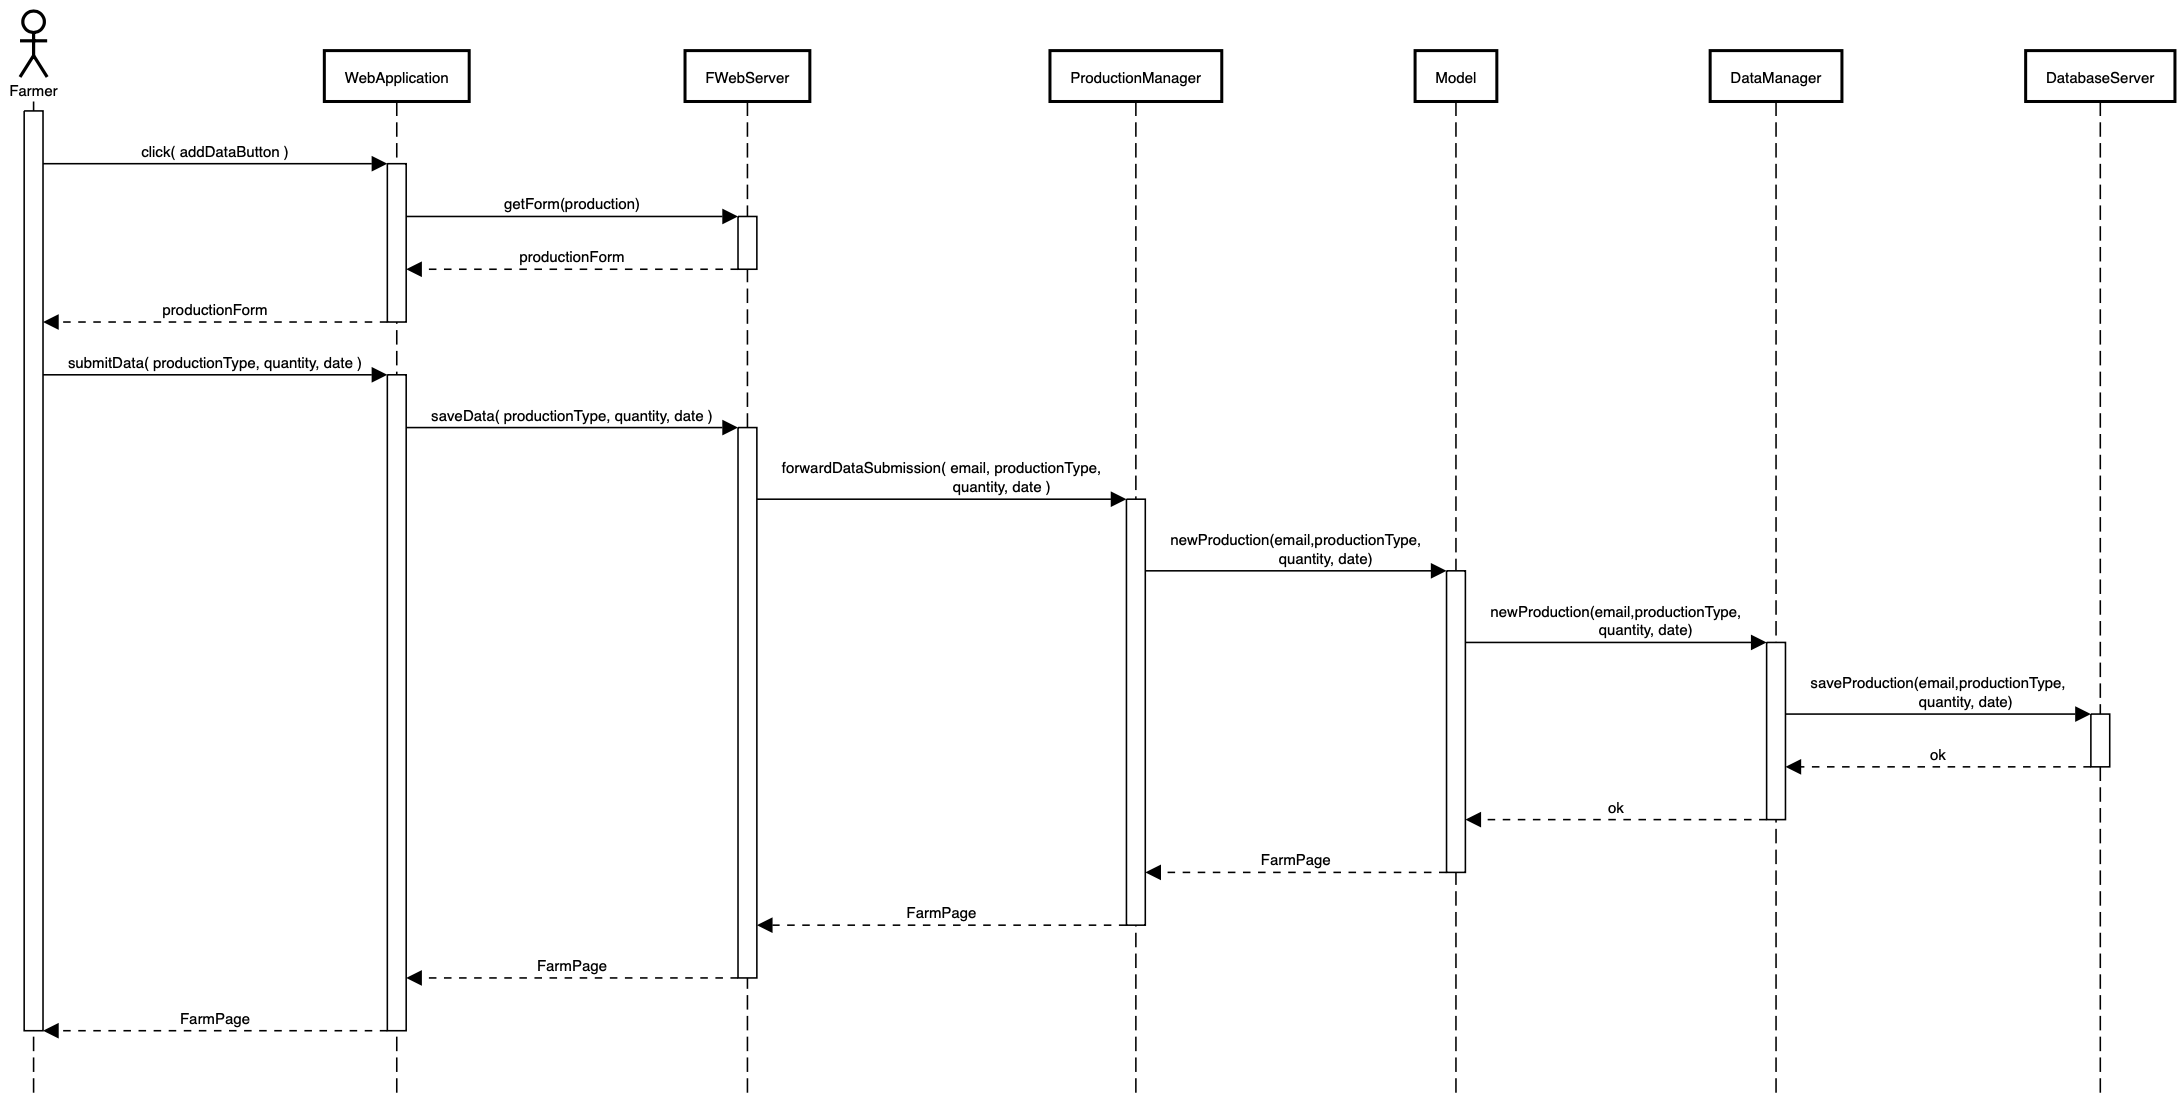
\includegraphics[width=0.7\textwidth]{sequance/addData-2.png}
        \caption{\emph{Submit production data} sequence diagram}
        \label{fig:sequence4}
        \end{center}
    \end{figure}
    \item \textbf{map visualization}\\
    Here is shown how the system provides the visualization of the map to the user, with different level of visibility based on their permission.
        \begin{itemize}
            \item the user is a farmer: the Model contruct the object that rapresenting the map filled with all the farms saved in the system and only the type of production that are producted in it.
            \item the user is a policy maker: the Model contruct the map object with the farms located on it with basic production data and the evaluetion of it.
        \end{itemize}
    From the Map page is possible, by a click on a specific button, for policy maker to evaluate a farm.
    \begin{figure}[H]
        \begin{center}
        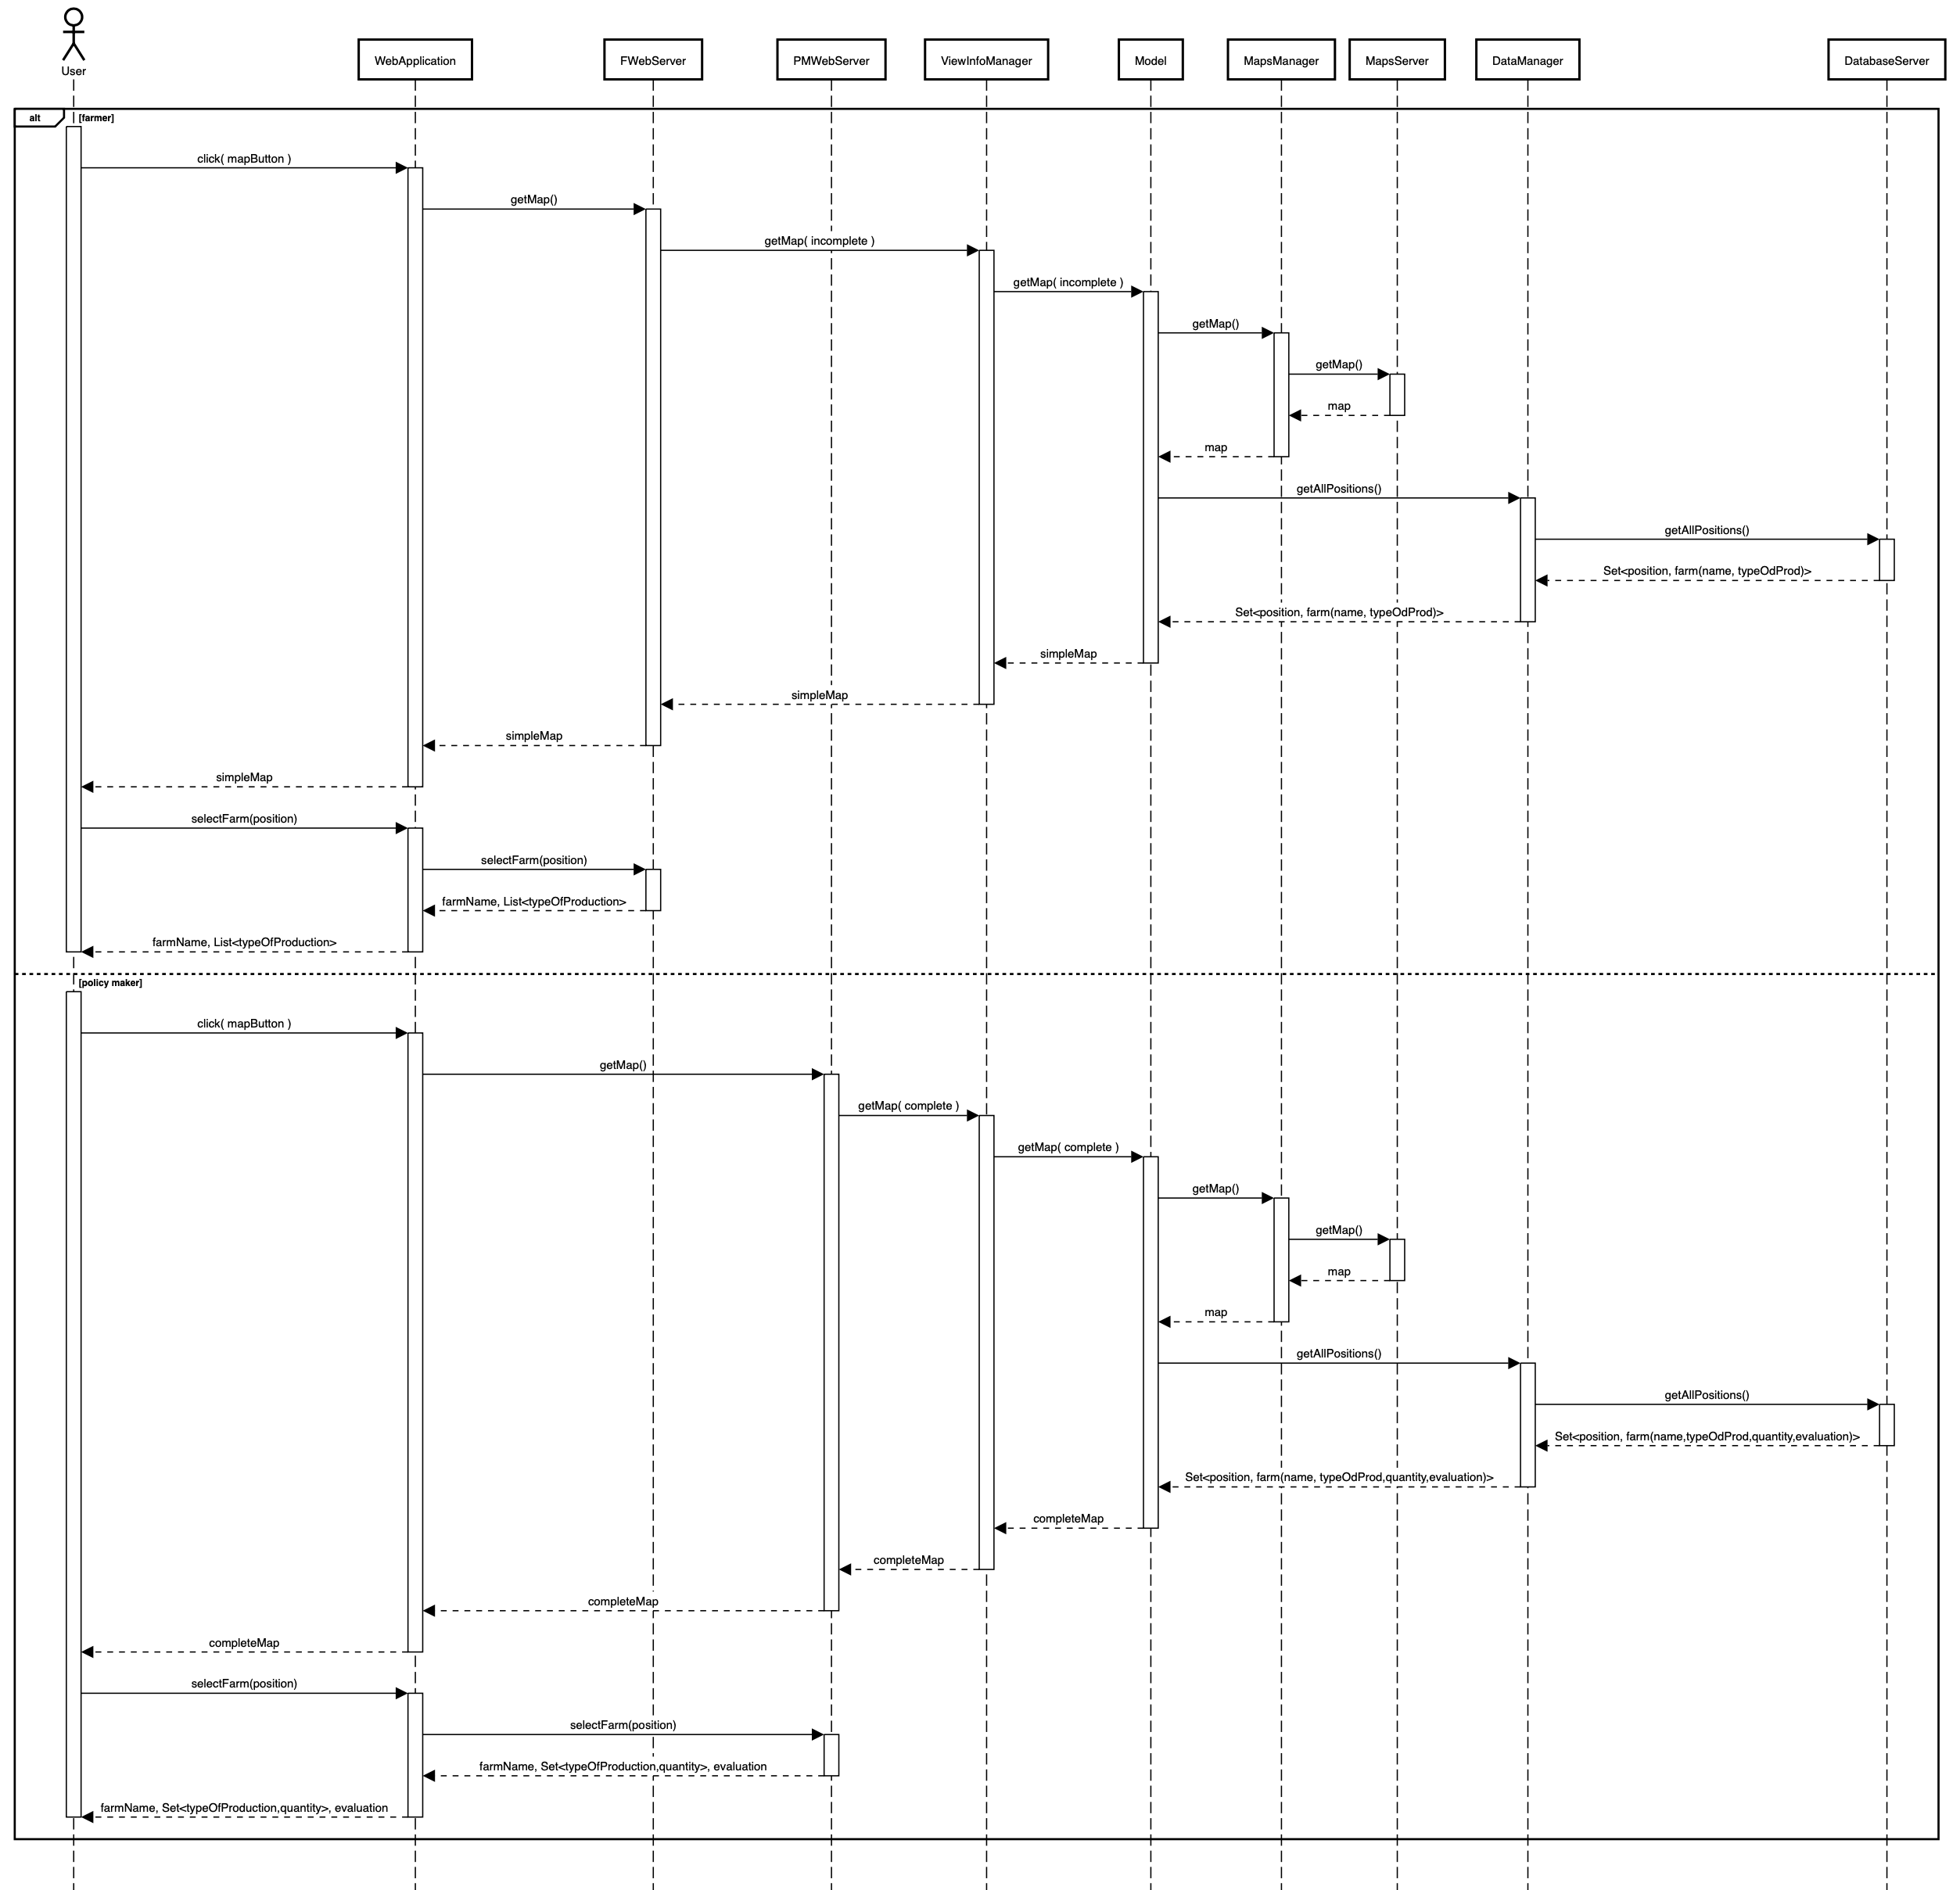
\includegraphics[width=0.7\textwidth]{sequance/viewMap.png}
        \caption{\emph{Visualize map} sequence diagram}
        \label{fig:sequence5}
        \end{center}
    \end{figure}
    \item \textbf{policy maker makes an evaluation}\\
    This diagram describes the process of evaluation a farmer by a policy maker. At first, when the day of the month in wich the evaluation must be done, the policy maker select from the map the farm that he wants to evaluate and he clicks on the 'Evaluate' button. His Web Server provides him the form to fill with the results of the evaluation, with already the addresse attached. When this notification is submitted by the policy maker, his web server forward it to the notification manager that deal with the enrollment of the result in the database and also send it to the farmer evaluated.
    \begin{figure}[H]
        \begin{center}
        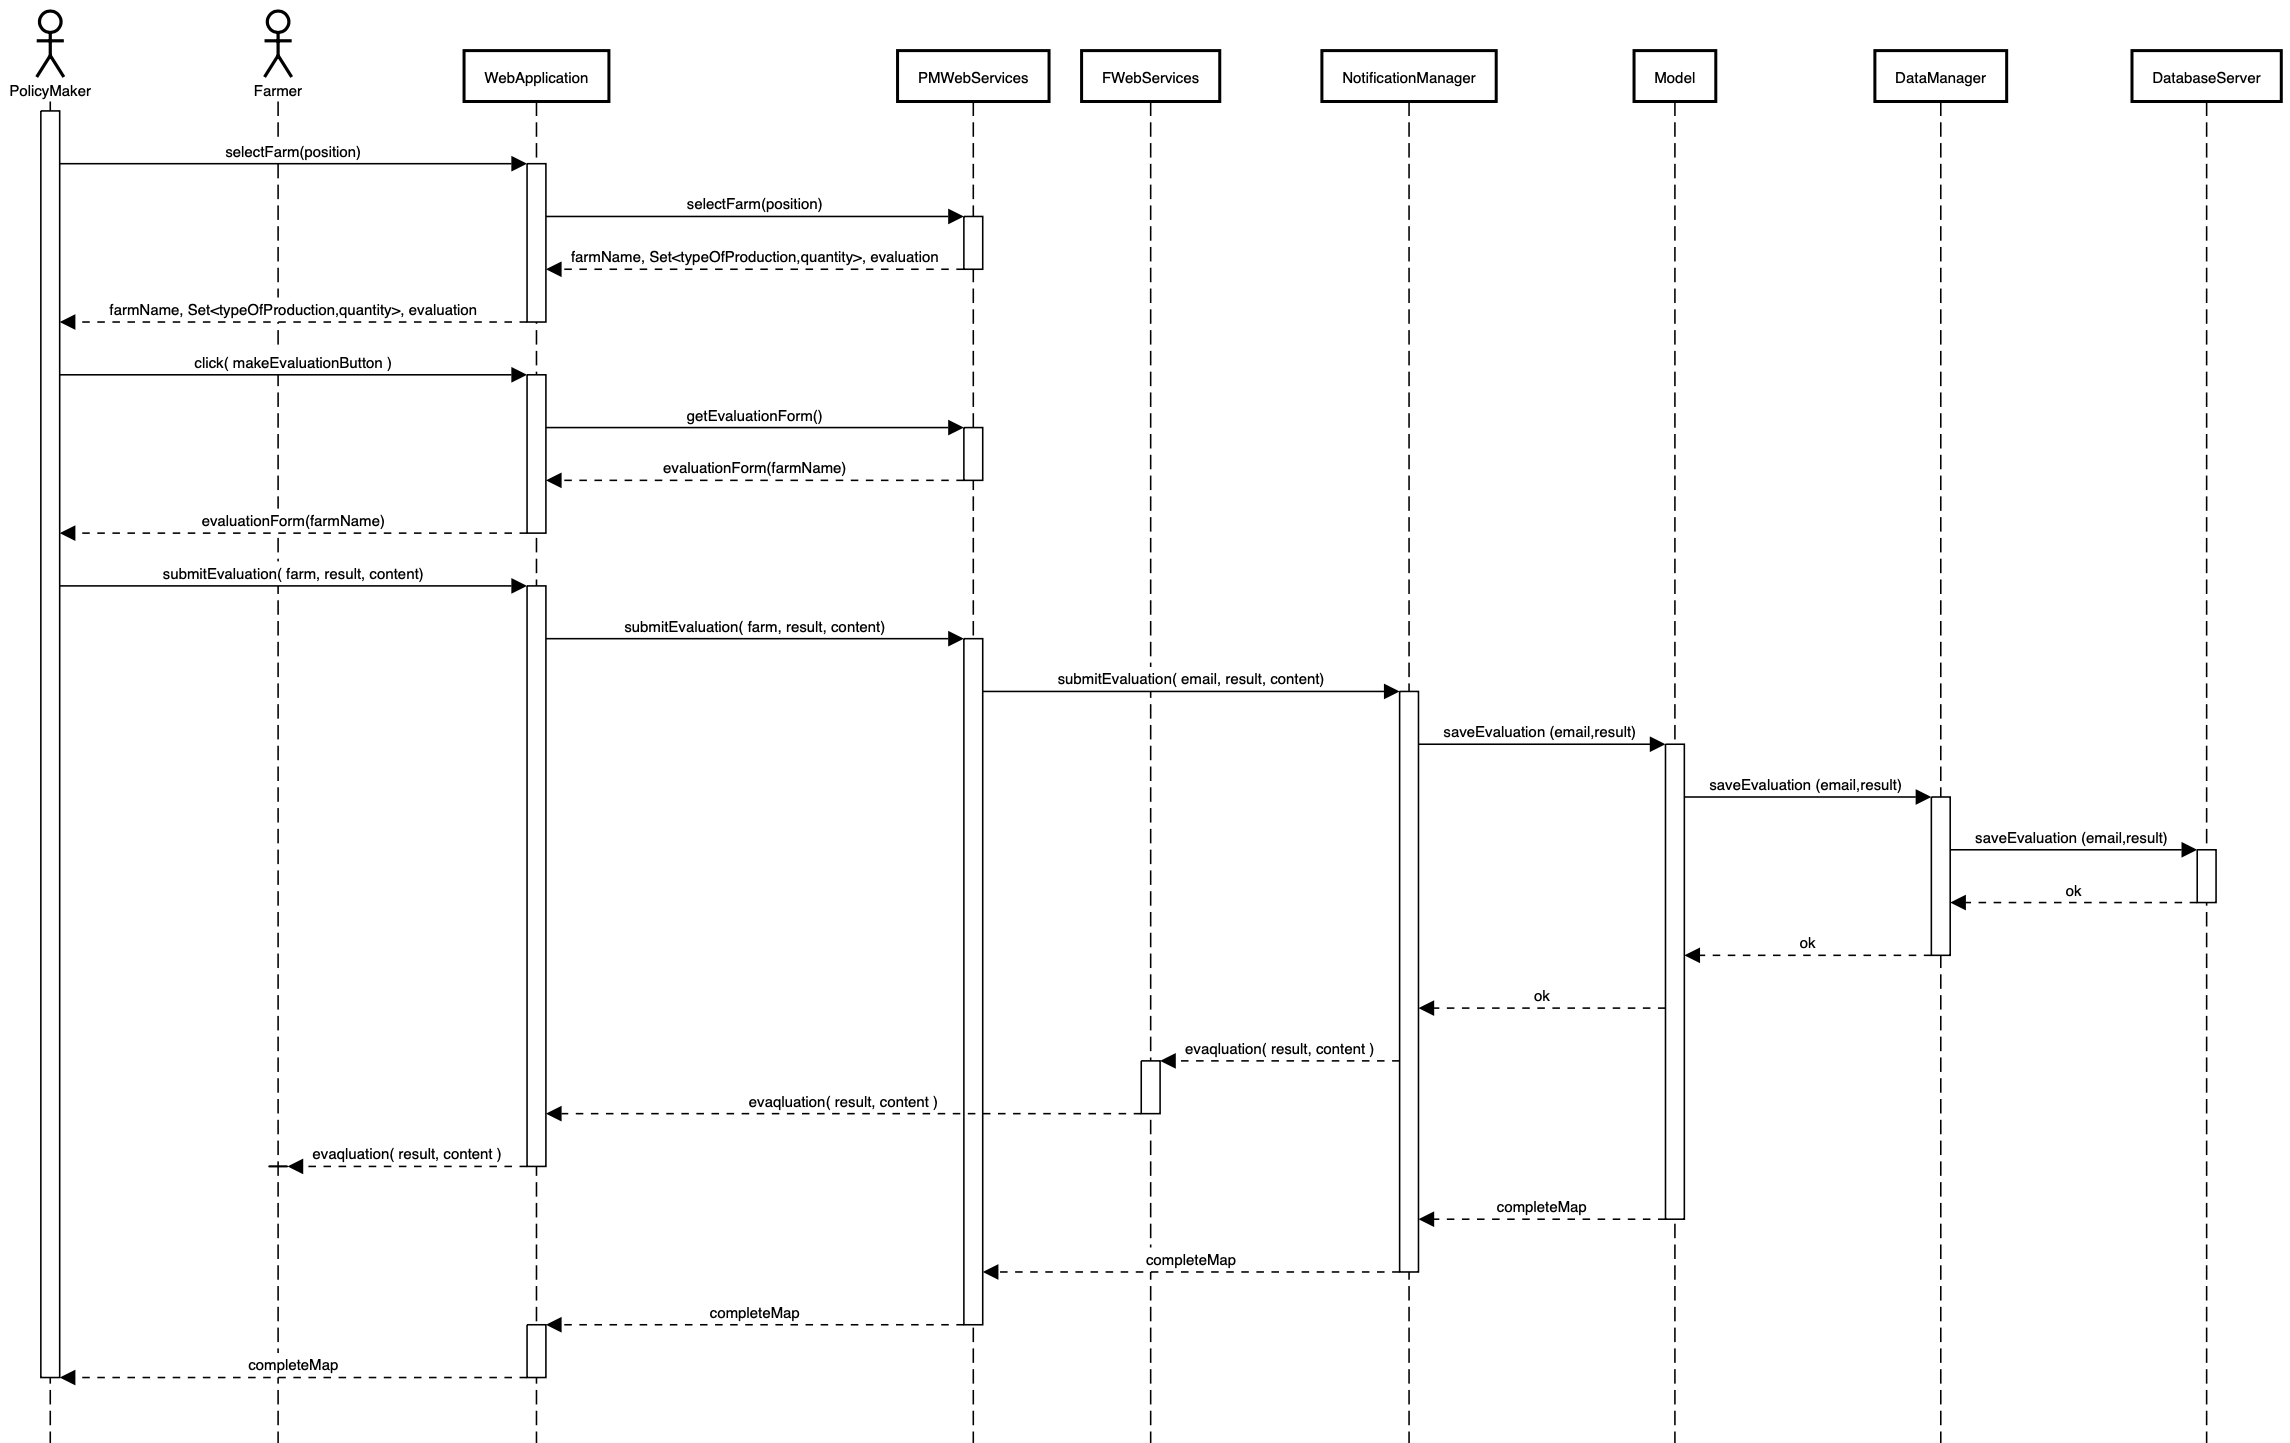
\includegraphics[width=0.7\textwidth]{sequance/updateMap.png}
        \caption{\emph{Make evaluation} sequence diagram}
        \label{fig:sequence6}
        \end{center}
    \end{figure}
    \item \textbf{farm's page visualization}\\
    This functionality is avaiilable for both users, the only differences are:
    \begin{itemize}
        \item a farmer has only a button on his home page that he clicks when wants to visualize his \textbf{own} farm page
        \item a policy maker has a form on which he writes the name of the farm he wants to visualize and pressing enter sends the request to the web application
        \item for the first user the received web page will have a button for the notification visualization and the buttons for the creation of  help and advice notification
    \end{itemize}
    After received the request, the web application sends it to the view info manager (by the user's server), that collects all the data from the model. The last component gets from the right database all the data to generate all the object rapresenting the page content:
    \begin{itemize}
        \item from the application database gets the farm basic information, such as name and surname of the farm's owner, the farm name, the email and the position (as coordinates)
        \item also from the application database it gets the production's information whith which create a set having as key the date and as value another key-value structure containing for each type of production the quantity crop 
        \item the third request to the application database is the one to get the sensors data, that these dispositives put automatically in the database and always related to a specific day and position (corresponding to the farm on which they work)
        \item it asks to the external system to retreive the weather information from the day of the request and all the ones befor in the position on the farm. This information are stored in a database specific of this system
    \end{itemize}
    After the model creates the structure for all the content of the page, forward them to the view info manager to the user's server and then the web application that will provide the visualization of these data.
    \begin{figure}[H]
        \begin{center}
        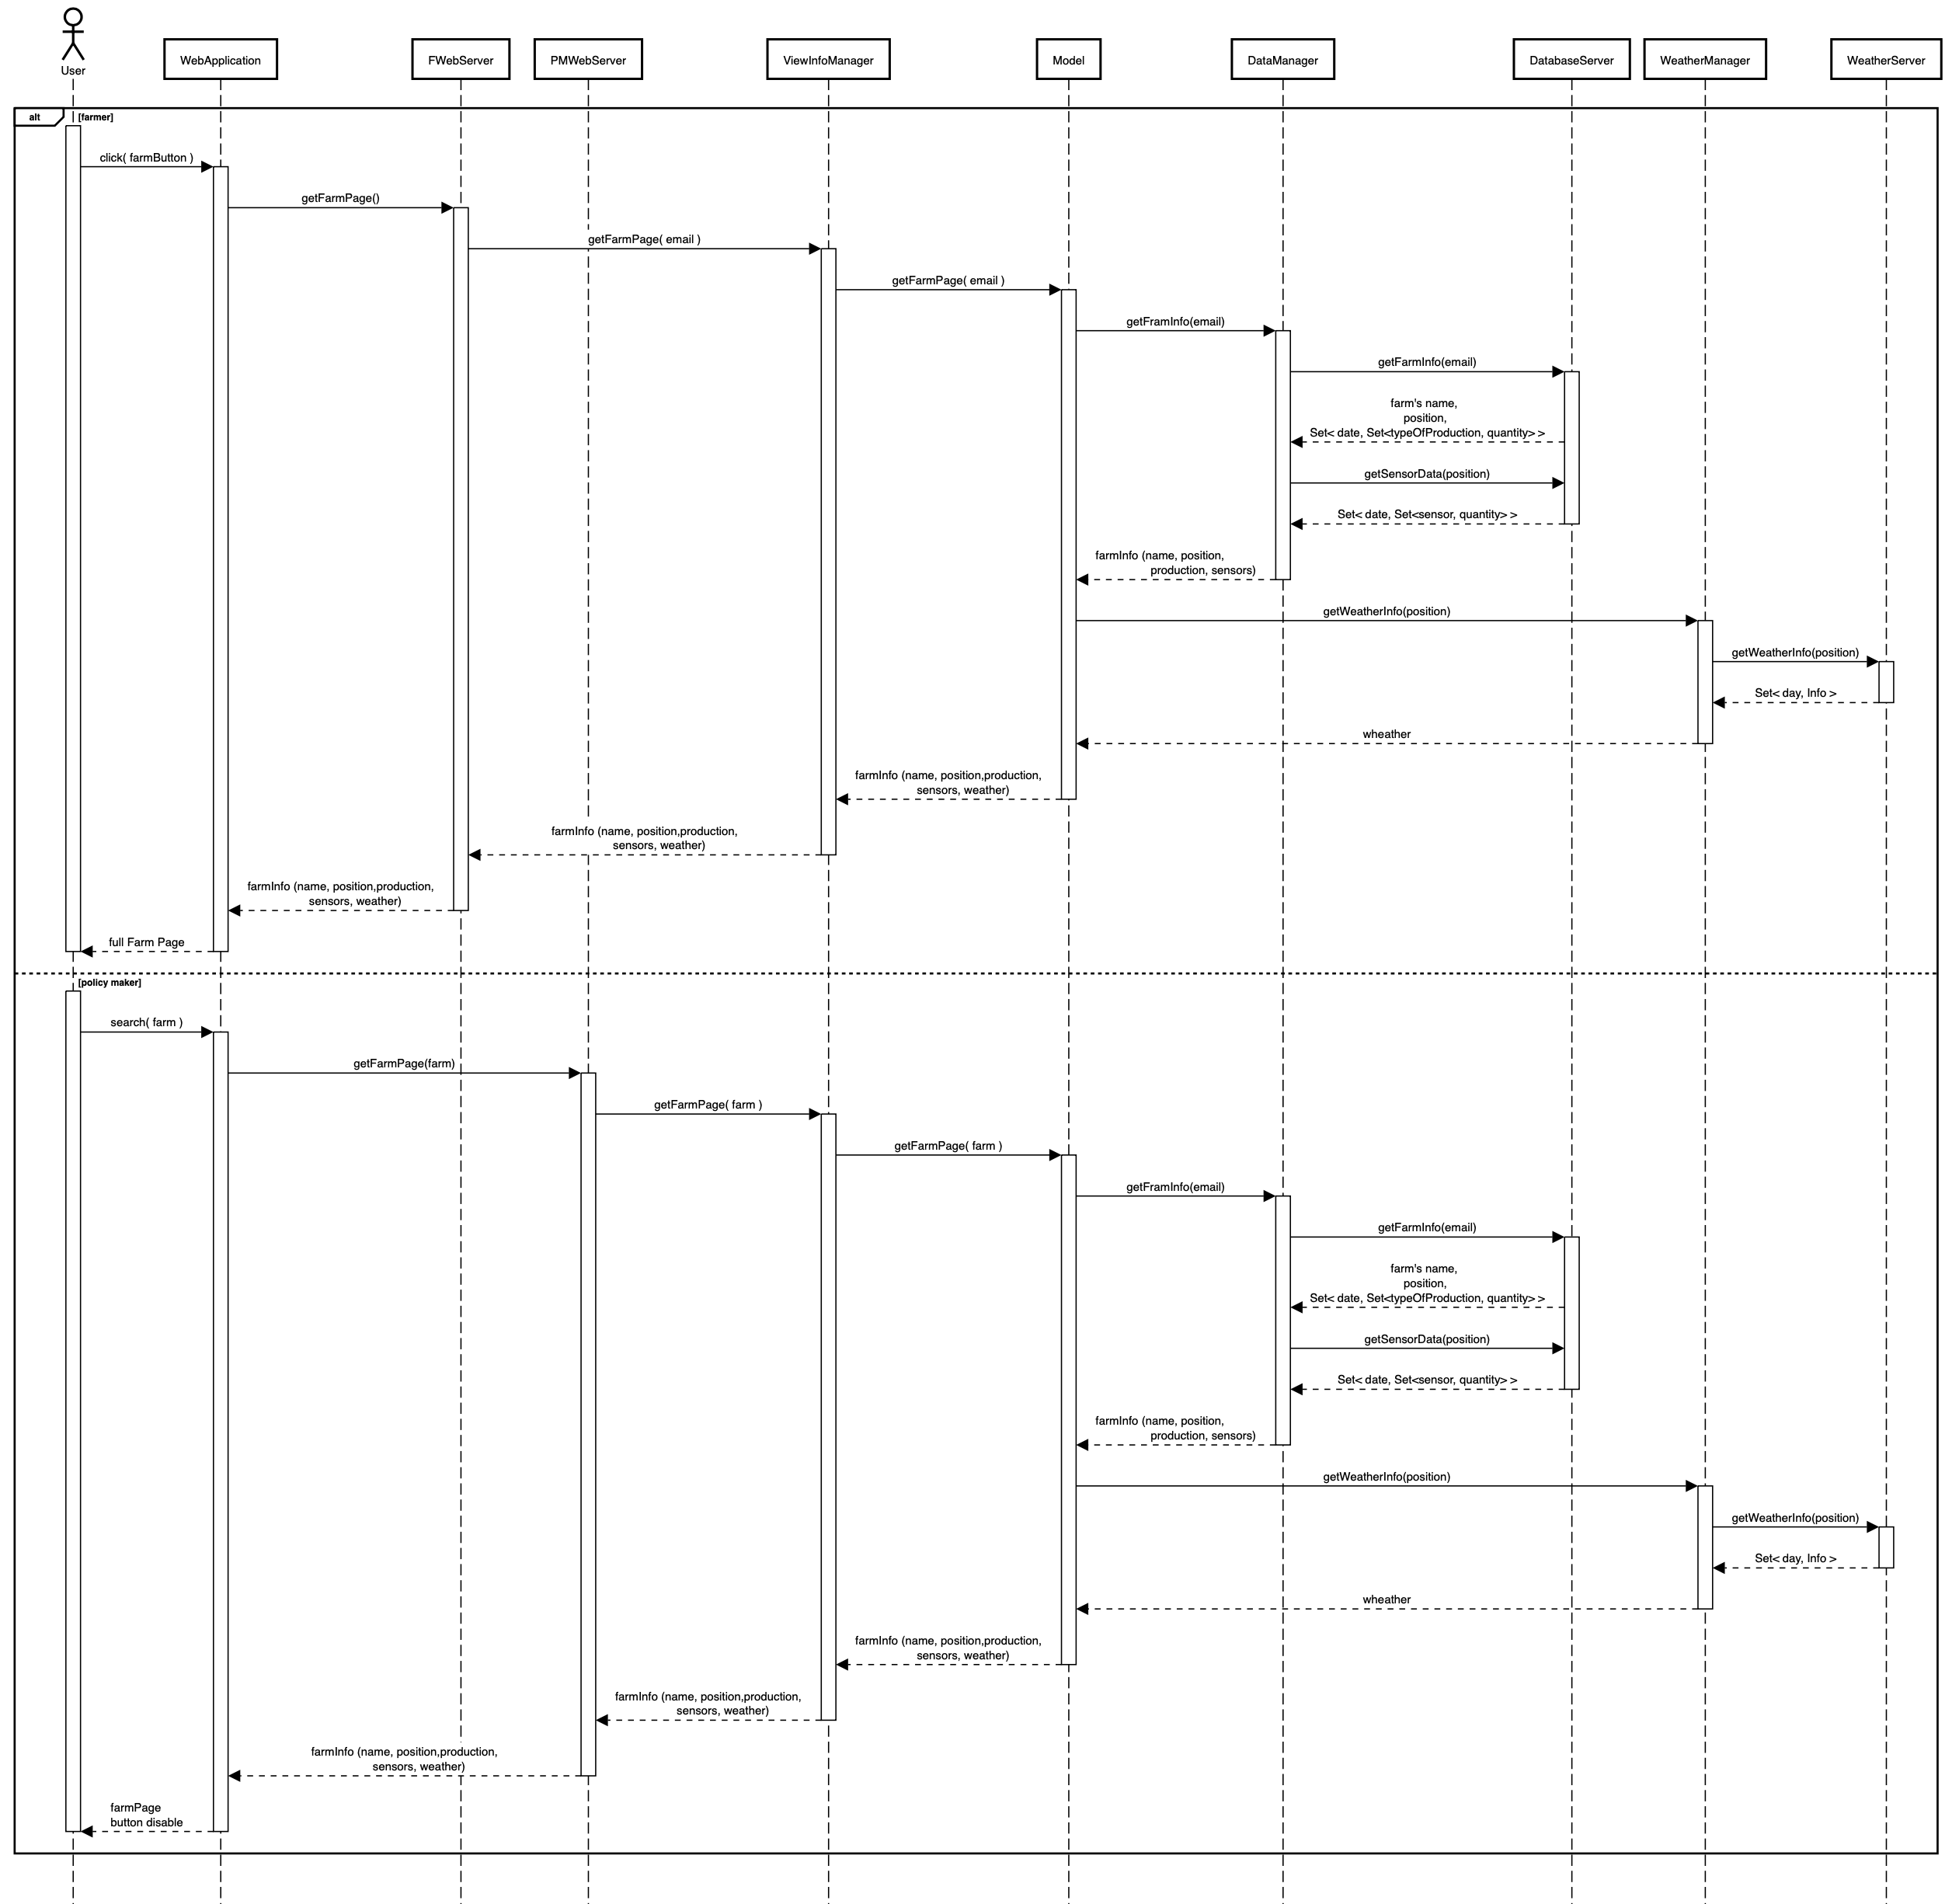
\includegraphics[width=0.7\textwidth]{sequance/farmPage.png}
        \caption{\emph{Visualize farm page} sequence diagram}
        \label{fig:sequence7}
        \end{center}
    \end{figure}
    \item \textbf{notification submittion}\\
    Different kind of notification can be sent in the system.
    \begin{itemize}
        \item advice: a farmer can select the advice button from his farm's page. He just have to select the type of production on which he wants to gave an advice and write it in the specific form. Will be the framer's server that will attach on it the references of the writer (the email of the farmer), and the date and time on which he submit the advice, before saving it in the database. Before push it in the database, the notification manager checks it the sender is a good farmer and if not just discard the notification.
        \item help: a farmer who wants to ask a formal request of help also select the help button on his farm's page. As the notification above he select the type and writes the content of the message, where specify the problem he's dealing with. In this case the notification does not need to be saved in a db but the notification manager selects randomly a policy maker as a recipient of it. 
        \item solution: a policy maker who received a request of help (process described above) can reply to it whith a solution. At first the user have to search the farm ho asks for it, and also all the avices stored in the system database about the type of production on which the problem is specified. Analyzing all these data he can  wrote some advice that should help the farmer with his problem and send him. In the moment when the policy maker selects the help notification on which he wants to respond and then submit it, the web application istantinelly attach the addresse (retreived by the sender of the help selected) and then the notification manager will forward it to him.
    \end{itemize}
    \begin{figure}[H]
        \begin{center}
        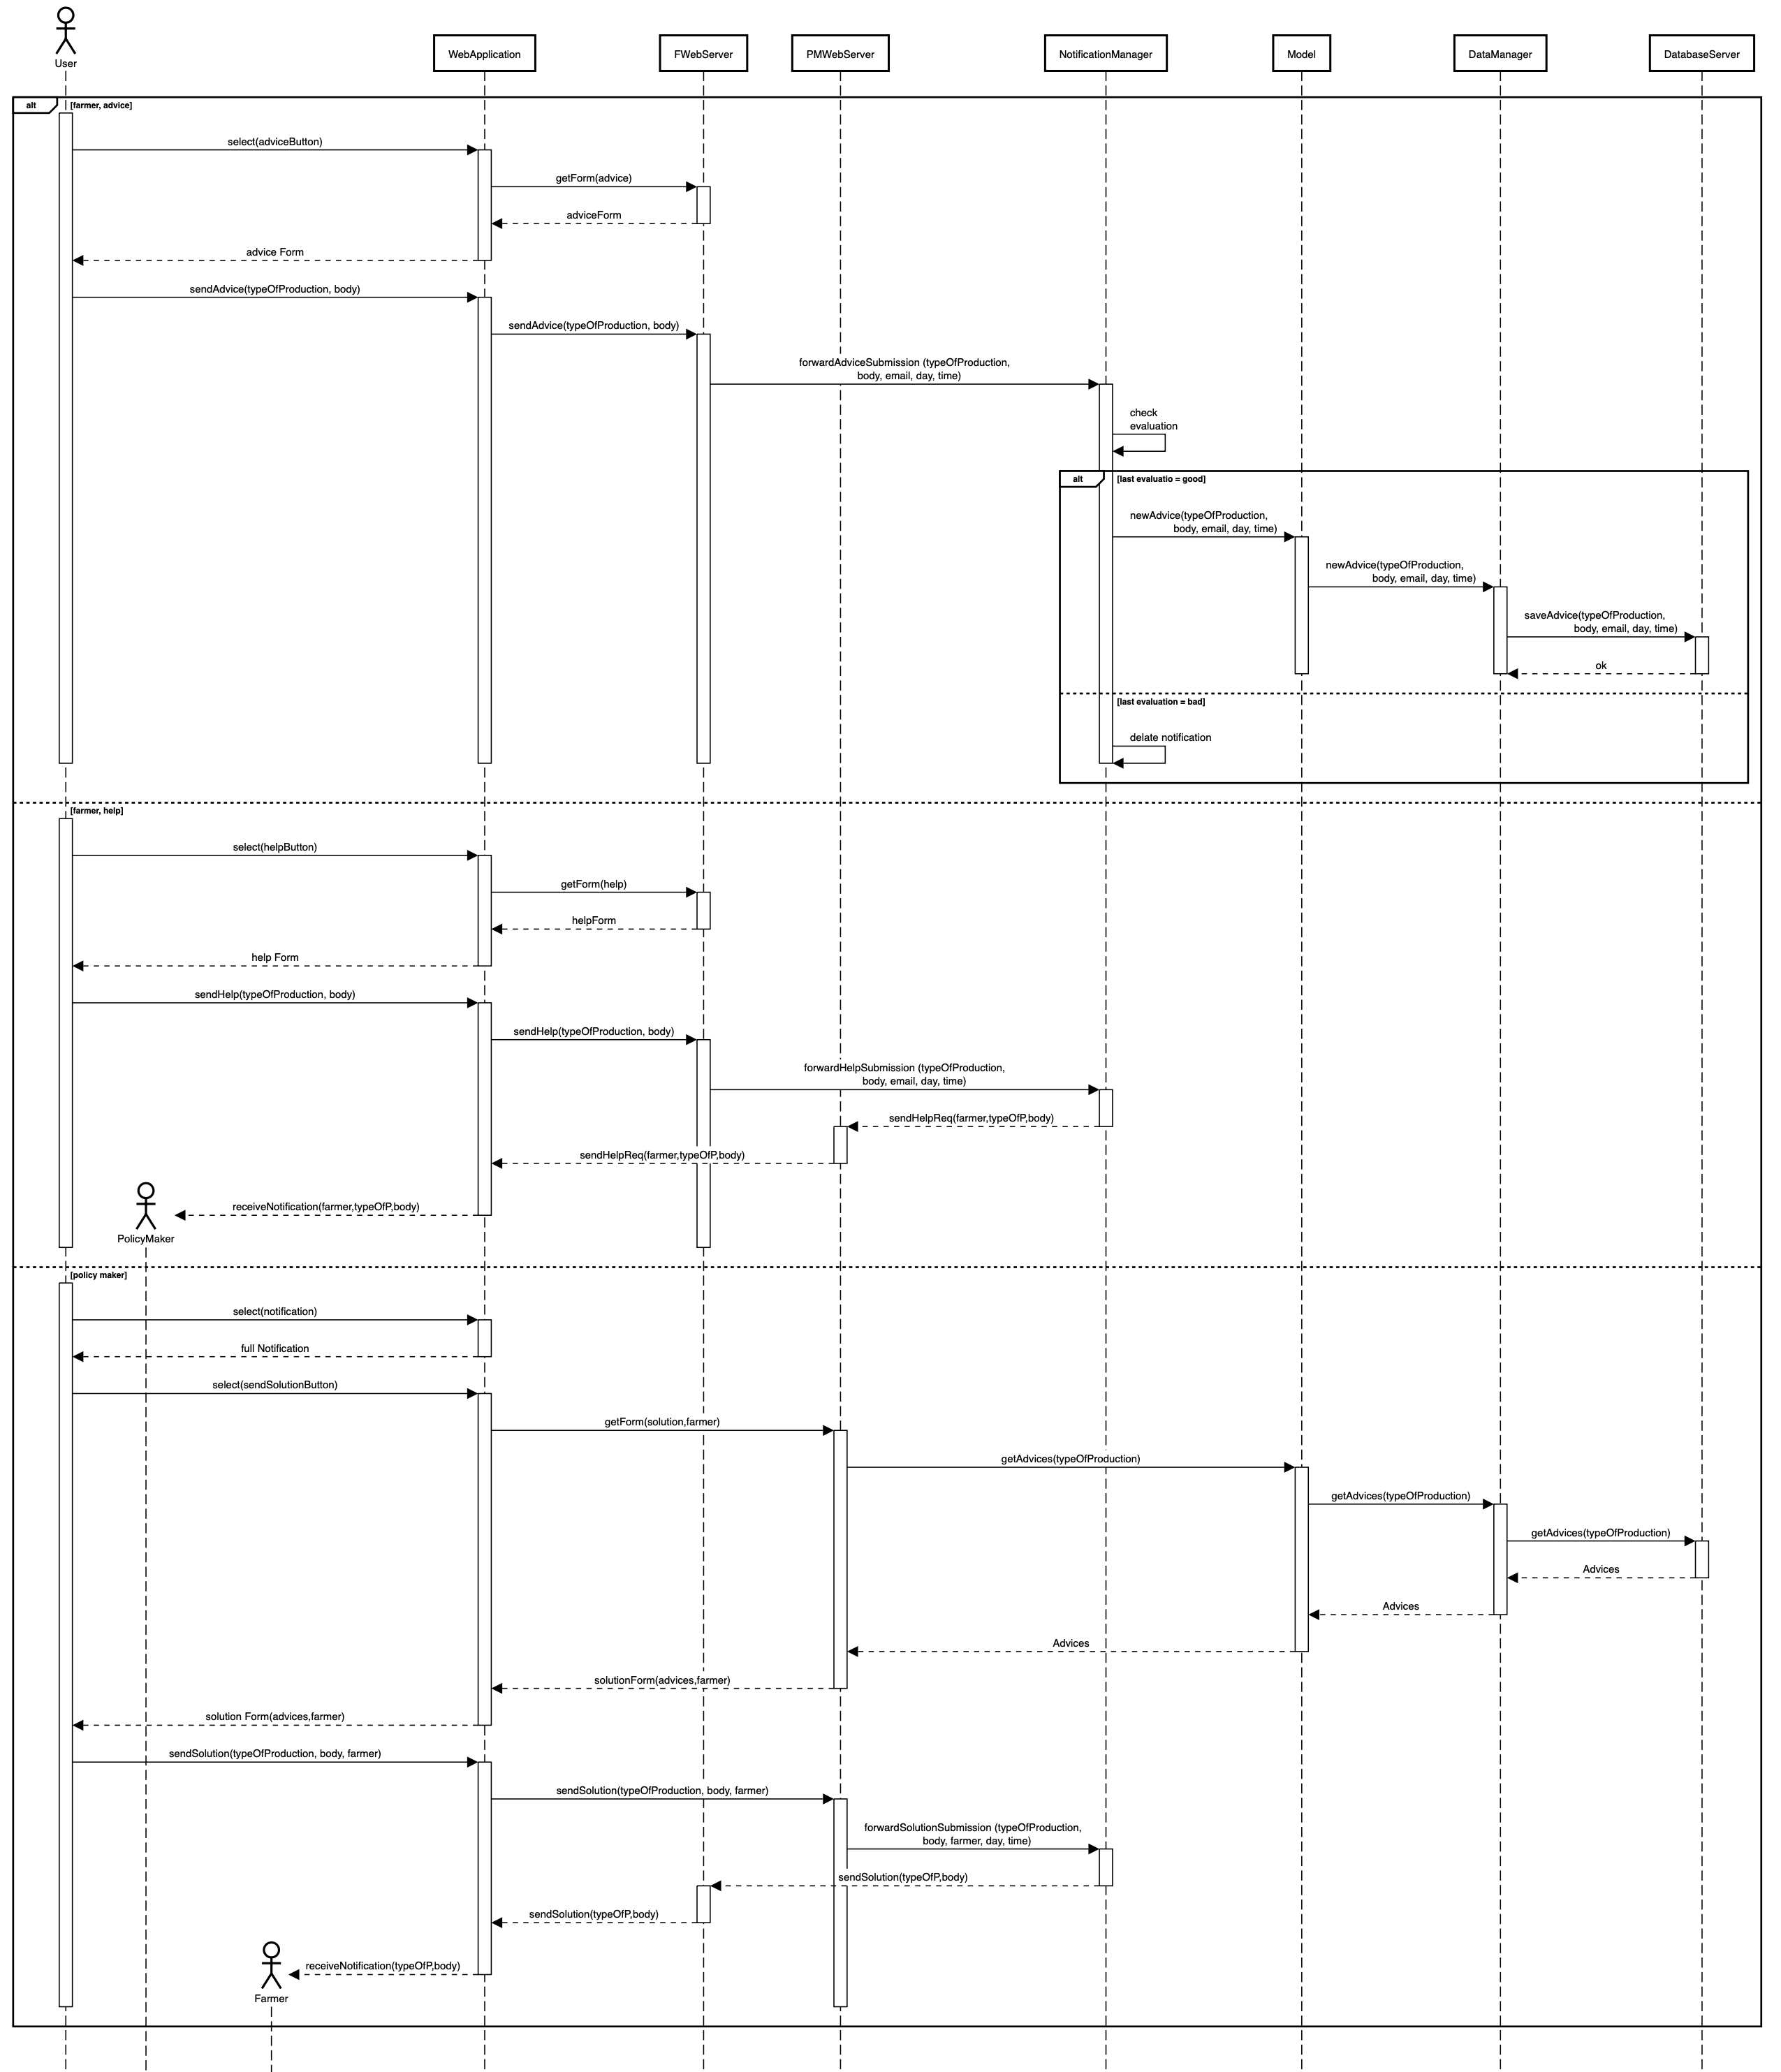
\includegraphics[width=0.7\textwidth]{sequance/sendNotifications.png}
        \caption{\emph{Send notifications} sequence diagram}
        \label{fig:sequence8}
        \end{center}
    \end{figure}
    \item \textbf{notification visualization}\\
    In this sequence is shown how the system provide the visualization of the notifications after a request of a user. For the farmer the process starts on his farm's page, where clicking the bell button send the request, dream server collect from the database all his notification. The model crete with the data the structure to be sent to the web application that provide the list to the user. All the messages are in the web application in that moment, so when he select one of the notifications in the list it provides the full content of it. on the other hand the policy maker to visualize his notifications starts from his home page and clicks on the specific button. The rest of the process is equal as for the farmer.
    \begin{figure}[H]
        \begin{center}
        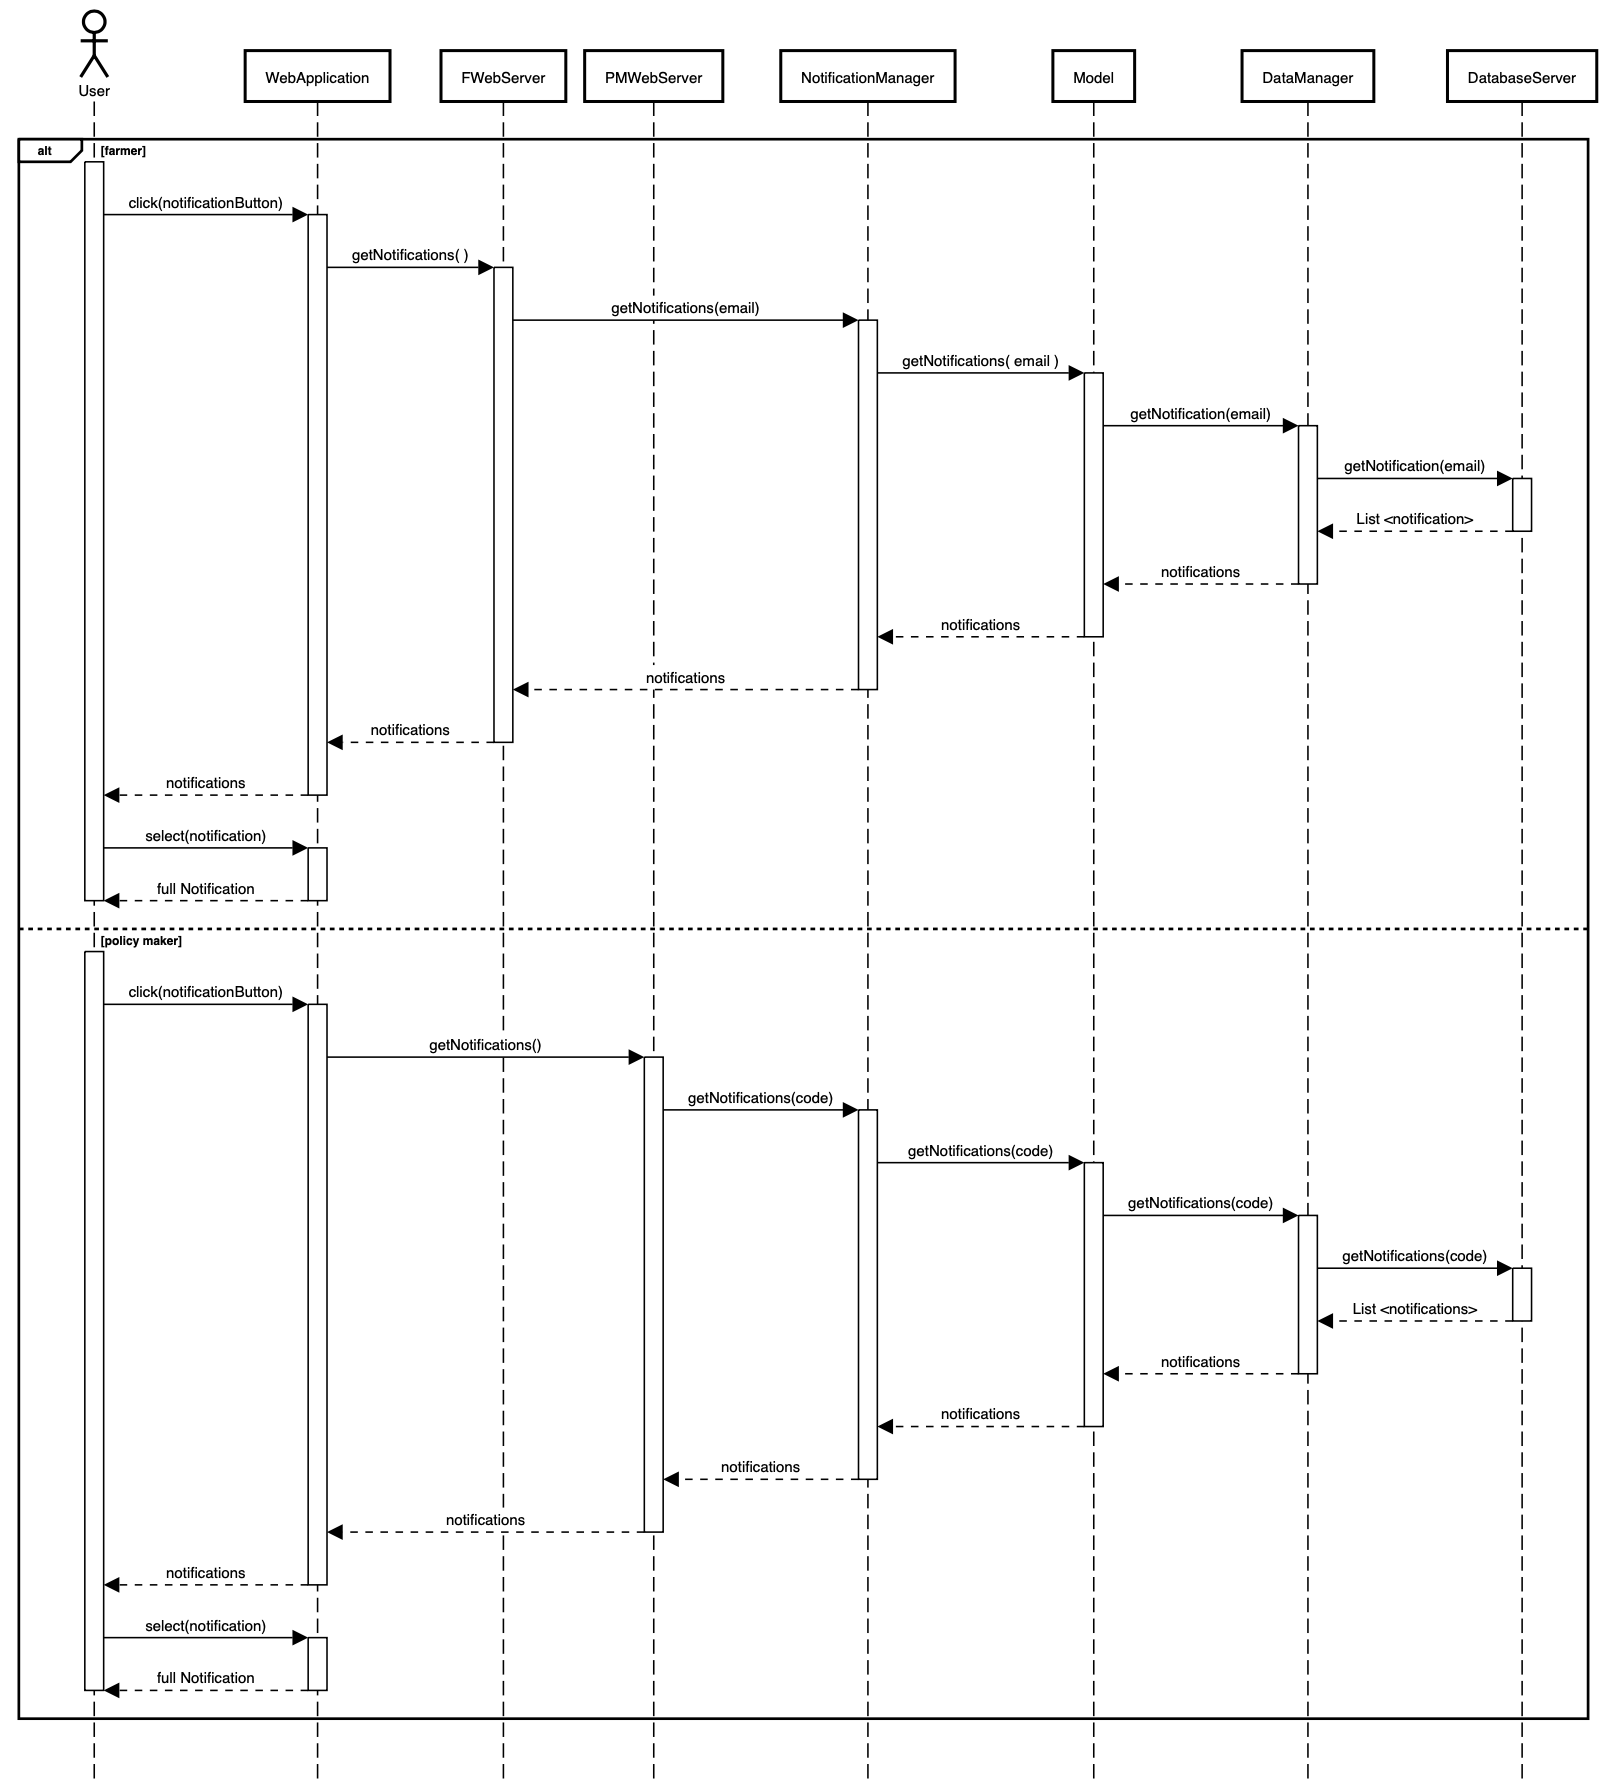
\includegraphics[width=0.7\textwidth]{sequance/viewNotifications.png}
        \caption{\emph{Visualize notifications} sequence diagram}
        \label{fig:sequence9}
        \end{center}
    \end{figure}
    
\end{enumerate}

%---------------------%
\subsection{Component interfaces}



%---------------------%
\subsection{Architectural styles and patterns}

%---------------------%
\subsection{Other design decisions}

